\section{Floquet (Trotterized) dynamics}
\label{sec:floquet}

The exact evolution $e^{\Lv t}$ (Sec.~\ref{sec:dissipation}) sums a Taylor series of the generator (sparse, or matrix-free for $L \ge 11$) at every step, and the trajectories a Taylor series of $e^{-iH\tau}$. A Trotterized step replaces both by a fixed circuit of 4-site gates: one step of $\rho$ costs $L\cdot 256\cdot 4^L$ multiply-adds (no generator is stored), one step of a trajectory $64\,L\,2^L$. This chapter defines the circuit (the same as \texttt{floquet-circuit.md} in the repository), shows it for $L = 8, 12$ (four layers) and $L = 10, 14$ (five and seven layers), checks it against the exact evolution, and uses it to recompute the depolarizing thermodynamic rates of Fig.~\ref{fig:chinf} up to $L = 24$ (Sec.~\ref{sec:floquet-dep}). Code: \texttt{rust/src/floquet.rs}, binaries \texttt{floquet} ($\rho$, $L \le 16$) and \texttt{floquet\_traj} (trajectories).

\subsection{Splitting of the Hamiltonian into blocks}
\label{sec:floquet-blocks}

Group the terms of $H_I$ by their singlet projector. The block of bond $(j+1, j+2)$ lives on the four sites $j, \dots, j+3$:
\begin{equation}
h_j = \underbrace{\sum_\alpha a_\alpha\, R_{j+1,j+2}\,\sigma^\alpha_{j+3}}_{\mathrm{RA}}
 + \underbrace{\sum_\alpha b_\alpha\, \sigma^\alpha_{j}\,R_{j+1,j+2}}_{\mathrm{AR}}
 + \underbrace{\sum_{\alpha\beta} c^{(j+1)}_{\alpha\beta}\, \sigma^\beta_{j}\,R_{j+1,j+2}\,\sigma^\alpha_{j+3}}_{\mathrm{ARA}},
\qquad H_I = \sum_{j=1}^{L} h_j ,
\label{eq:floquet-block}
\end{equation}
with the coefficients of Sec.~\ref{sec:model} (the random $c$ stays attached to its physical bond). The three families occupy the sites
\begin{center}
\begin{tabular}{lcccc}
\toprule
term & site $j$ & $j+1$ & $j+2$ & $j+3$ \\
\midrule
RA  & $\mathds 1$ & $R$ & $R$ & $A$ \\
AR  & $A$ & $R$ & $R$ & $\mathds 1$ \\
ARA & $A$ & $R$ & $R$ & $A$ \\
\bottomrule
\end{tabular}
\end{center}
where the two entries $R$ are the two ends of one projector $R_{j+1,j+2} = (\mathds 1 - \sigma^x\sigma^x - \sigma^y\sigma^y - \sigma^z\sigma^z)/4$ and $A$ a single-site Pauli factor. Every term of $h_j$ is $R_{j+1,j+2}$ times an operator on the outer sites $j, j+3$, which commutes with it, so $h_j\ket{\Phi_n} = 0$ for every tower state: each block annihilates the tower on its own, and so does each block gate $e^{-i\Delta t\, h_j}$ act as the identity on it.

\subsection{Layers}
\label{sec:floquet-layers}

Blocks that share a site do not commute, so the $L$ blocks are distributed over $d$ layers of disjoint blocks:
\begin{equation}
\begin{gathered}
d = \min\{\, d' \ge 4 : d' \text{ divides } L \,\}, \\
\text{layer } U_\ell \ (\ell = 1, \dots, d):\ \text{blocks starting at } j = \ell,\ \ell + d,\ \dots,\ \ell + (L/d - 1)\,d .
\end{gathered}
\label{eq:floquet-layers}
\end{equation}
The spacing $d \ge 4$ keeps the blocks of a layer disjoint, and since $d$ divides $L$ the pattern closes around the ring: every layer is the previous one shifted by one site, each layer has $L/d$ blocks and $d - 4$ idle sites after every block, and every site starts exactly one block per step, so every bond is the middle bond of exactly one block and every term of $H_I$ appears once with its full coefficient. $d = 4$ whenever $4 \mid L$; otherwise $d$ is the smallest divisor above 4 ($L = 6$: 6, $L = 10$: 5, $L = 14$: 7, $L = 18$: 6, $L$ prime: $L$). The block starts of the four examples (idle sites in parentheses):
\begin{center}
\small\setlength{\tabcolsep}{5pt}
\begin{tabular}{lllll}
\toprule
layer & $L = 8$ & $L = 10$ & $L = 12$ & $L = 14$ \\
\midrule
$U_1$ & 1, 5 & 1, 6 \ (5, 10) & 1, 5, 9 & 1, 8 \ (5, 6, 7, 12, 13, 14) \\
$U_2$ & 2, 6 & 2, 7 \ (1, 6) & 2, 6, 10 & 2, 9 \ (6, 7, 8, 13, 14, 1) \\
$U_3$ & 3, 7 & 3, 8 \ (2, 7) & 3, 7, 11 & 3, 10 \ (7, 8, 9, 14, 1, 2) \\
$U_4$ & 4, 8 & 4, 9 \ (3, 8) & 4, 8, 12 & 4, 11 \ (8, 9, 10, 1, 2, 3) \\
$U_5$ & -- & 5, 10 \ (4, 9) & -- & 5, 12 \ (9, 10, 11, 2, 3, 4) \\
$U_6$ & -- & -- & -- & 6, 13 \ (10, 11, 12, 3, 4, 5) \\
$U_7$ & -- & -- & -- & 7, 14 \ (11, 12, 13, 4, 5, 6) \\
\bottomrule
\end{tabular}
\end{center}
Since the Trotter error depends on the layering, a scan in $L$ should use sizes divisible by 4 (the same circuit at every $L$).

\subsection{One step}
\label{sec:floquet-step}

One step of length $\Delta t$ applies the interaction layers (from $U_d$ to $U_1$), then the field on every site, then the noise on every site:
\begin{equation}
F = \mathcal E \circ \mathcal B \circ \mathcal U_1 \circ \mathcal U_2 \circ \dots \circ \mathcal U_d, \qquad
\mathcal U_\ell(\rho) = U_\ell\,\rho\,U_\ell^\dagger, \quad U_\ell = \prod_{j \in \ell} e^{-i\Delta t\, h_j}, \qquad
\rho(N\Delta t) = F^N \rho(0),
\label{eq:floquet-step}
\end{equation}
(the rightmost map acts first) with the uniform field and the noise
\begin{equation}
\mathcal B(\rho) = U_B\,\rho\,U_B^\dagger, \quad U_B = \prod_{j=1}^{L} e^{-i\frac h2 \Delta t\, \sigma^z_j} = e^{-ih\Delta t\, S^z_{\mathrm{tot}}}, \qquad
\mathcal E = \bigotimes_{j=1}^{L} e^{\Delta t\, \D_j} .
\label{eq:floquet-field-noise}
\end{equation}
$U_\ell$ is exact because the blocks of a layer commute. The noise is \emph{one} layer for any $L$ and any $d$: the dissipators $\D_j$ of different sites act on different sites and commute, so $e^{\Delta t \sum_j \D_j} = \bigotimes_j e^{\Delta t\, \D_j}$ exactly. For a Hermitian Pauli channel (\texttt{floquet.rs} accepts $\sigma^z$, $\sigma^x$, $\sigma^y$, dep, depol and xyz) $e^{\Delta t\, \D_j}$ is diagonal in the Pauli basis: for $\sigma^z$ dephasing it multiplies the $\sigma^x_j$ and $\sigma^y_j$ components of $\rho$ by $e^{-2\gamma\Delta t}$ and leaves $\mathds 1$, $\sigma^z_j$ unchanged. The circuit has depth $d + 2$ ($d$ interaction layers, one field layer, one noise layer). The only approximation is the splitting: $F = e^{\Delta t\, \Lv} + O(\Delta t^2)$ per step, from the commutators of the layers with each other, with $S^z_{\mathrm{tot}}$ and with $\D$, so an error $O(\Delta t)$ at fixed $t$ (first order). The output step of the binaries is the Trotter step $\Delta t \cdot \min(1, 0.5/\gamma)$.

\paragraph{The tower is exact at $\gamma = 0$.} Every block gate is the identity on the tower (Sec.~\ref{sec:floquet-blocks}) and $U_B\ket{\Phi_n} = e^{-ih\Delta t(L/2 - n)}\ket{\Phi_n}$, so $F^N$ reproduces reference~1 (the precessing product state, $\langle\sigma^x_j\rangle = -\cos ht$, $\langle\sigma^y_j\rangle = -\sin ht$) exactly for any $\Delta t$; the Trotter error acts only outside the tower, and on the scar only after the noise has moved weight out of it. Test \texttt{floquet\_scar\_oscillations\_are\_exact}: deviation $< 10^{-12}$ over 100 steps of $\Delta t = 0.3$ for $\rho$ at $L = 6, 8$ and for the state vector at $L = 6, 8, 10, 14$.

\paragraph{Why the field is a separate layer.} A first version applied the field inside the blocks, $e^{-i\Delta t\, h_j}e^{-i\frac h2\Delta t\,\sigma^z_j}$ on the start site of every block (also one rotation per site per step). Then the spins precess at different times: when a block of layer $d - 1$ acts, its middle site $j + 1$ has already been rotated (in layer $d$) and $j + 2$ not yet (layer 1), so the two ends of $R_{j+1,j+2}$ differ by the angle $h\Delta t$ and $R$ no longer annihilates the product state (singlet overlap $\approx h\Delta t/2\sqrt2$). With one rotation per site distributed over the layers some layer always sits at this seam, because the layer order is linear and the ring is cyclic. The error is first order and vanishes as $\Delta t \to 0$ (at $L = 8$, $\gamma = 0$: largest deviation from reference~1 over $t \le 6$ $0.100$, $0.049$, $0.024$ at $\Delta t = 0.2, 0.1, 0.05$, mostly a shift of the precession phase; $m_\perp(t = 50) = 0.9953$ at $\Delta t = 0.1$), but it breaks the scar at every finite $\Delta t$, while the uniform field layer keeps it exact. That version was not kept.

\subsection{Implementation}
\label{sec:floquet-impl}

The field and the noise of site $s$ commute with every gate that does not contain $s$. They are therefore folded into the \emph{last} gate applied that contains $s$ (layer 1 first, then 2, \dots; an idle site of $U_1$ goes into a gate of a lower layer), after its interaction, and the product of the $L$ gates is $F$ exactly. With $S_j$ the sites folded into block $j$, the unitary part of gate $j$ is $w_j = e^{-i\frac h2\Delta t\sum_{s\in S_j}\sigma^z_s}\,e^{-i\Delta t\, h_j}$ (a $16\times16$ matrix, exponentiated once).
\begin{itemize}
\item $\rho$ (\texttt{Floquet}, full Pauli basis $r_P = \Tr\rho P$): gate $j$ is the real $256\times256$ matrix
\[
G_j[P', P] = \prod_{s\in S_j} e^{\gamma\Delta t\, d(P'_s)}\ \Tr(P' w_j P w_j^\dagger)/16
\]
on the Pauli labels $P, P'$ of sites $j \dots j+3$, with $d(P'_s)$ the damping rate of the factor of $P'$ on site $s$ (noise after the unitary). $F$ ($4^L\times 4^L$) is never formed. Cost $L\cdot256\cdot4^L$ multiply-adds per step, memory $8\,\mathrm B\cdot4^L$ ($L = 16$: 34 GB); laptop (8 threads): 0.006, 0.034, 0.59 s per step at $L = 8, 10, 12$.
\item Trajectories (\texttt{FloquetTraj}): gate $j$ is the $16\times16$ unitary $\prod_{s\in S_j}\kappa_s\, w_j$, with $\kappa_s = e^{-i\theta_x\sigma^x_s}e^{-i\theta_y\sigma^y_s}e^{-i\theta_z\sigma^z_s}$, $\theta_\alpha \sim N(0, r_\alpha\gamma\Delta t)$ for a jump $\sqrt{r_\alpha\gamma}\,\sigma^\alpha$. On average $e^{-i\theta\sigma^\alpha}\rho\, e^{i\theta\sigma^\alpha}$ damps the two Pauli factors that anticommute with $\sigma^\alpha$ by $E[\cos2\theta] = e^{-2r_\alpha\gamma\Delta t}$, which is $e^{\Delta t\,\D}$ of that jump exactly, so the trajectory average is $F^N\rho(0)$ for any $\Delta t$ with statistical error only (test \texttt{floquet\_trajectories\_match\_floquet\_rho}). Cost $64\,L\,2^L$ real multiply-adds per step and trajectory, memory $16\,\mathrm B\cdot 2^L$.
\end{itemize}
The earlier protocol (commit \texttt{f223cc3}; its runs of 2026-11-24 are now in \texttt{data/non\_used\_data/}\allowbreak\texttt{floquet\_old\_protocol/}) used the smallest disjoint spacing (not a shift pattern, e.g.\ 5 layers at $L = 14$) and applied field and noise \emph{first}, folded into the first gate of every site. It keeps the scar exact as well; both protocols are first order and differ at $O(\Delta t)$ (Fig.~\ref{fig:floquet-checks}\,d).

\subsection{The circuits for $L = 8, 12$ and $L = 10, 14$}
\label{sec:floquet-circuits}

Figures~\ref{fig:floquet-circuit-8}--\ref{fig:floquet-circuit-14} show one step. Sites are fixed vertical wires, time runs upward: $U_d$ at the bottom acts first, $U_1$ last among the interaction layers, then the field row $U_B$ (one $B = e^{-i\frac h2\Delta t\,\sigma^z}$ on every wire) and the noise row $\mathcal E$ (one $\mathcal E_j$ on every wire). Inside each layer the rows RA, AR, ARA show the three summands of each block exponential $e^{-i\Delta t\, h_j}$ (one gate, not three), each capsule spanning the wires its term touches. A block that crosses the boundary between sites $L$ and 1 is cut at the two edges of the drawing (dashed ends, label repeated); idle sites of a layer are marked by dashed outlines. Each layer contains $L/d$ capsules of each family and every wire is idle in exactly $d - 4$ layers. The drawings are generated from the same rule as the code (\texttt{plot\_scripts/floquet\_circuit\_tikz.py}).

\begin{figure}[H]
\centering
\resizebox{0.62\textwidth}{!}{% One period of the Floquet circuit, N = 8, d = 4 interaction layers, then the uniform field and the noise (plot_scripts/floquet_circuit_tikz.py).
\begin{tikzpicture}[x=0.78cm, y=1cm]
\draw[black!35, line width=0.5pt] (1,-0.25) -- (1,8.54);
\node[font=\scriptsize, below] at (1,-0.25) {1};
\draw[black!35, line width=0.5pt] (2,-0.25) -- (2,8.54);
\node[font=\scriptsize, below] at (2,-0.25) {2};
\draw[black!35, line width=0.5pt] (3,-0.25) -- (3,8.54);
\node[font=\scriptsize, below] at (3,-0.25) {3};
\draw[black!35, line width=0.5pt] (4,-0.25) -- (4,8.54);
\node[font=\scriptsize, below] at (4,-0.25) {4};
\draw[black!35, line width=0.5pt] (5,-0.25) -- (5,8.54);
\node[font=\scriptsize, below] at (5,-0.25) {5};
\draw[black!35, line width=0.5pt] (6,-0.25) -- (6,8.54);
\node[font=\scriptsize, below] at (6,-0.25) {6};
\draw[black!35, line width=0.5pt] (7,-0.25) -- (7,8.54);
\node[font=\scriptsize, below] at (7,-0.25) {7};
\draw[black!35, line width=0.5pt] (8,-0.25) -- (8,8.54);
\node[font=\scriptsize, below] at (8,-0.25) {8};
\node[font=\scriptsize, below] at (4.50,-0.6) {site};
\draw[-latex, line width=0.6pt] (-2.35,0) -- (-2.35,8.54) node[midway, rotate=90, above, font=\scriptsize] {time};
\draw[decorate, decoration={brace, amplitude=4pt}, line width=0.6pt] (-0.95,0.05) -- (-0.95,1.21) node[midway, left=5pt, font=\small] {$U_{4}$};
\node[font=\tiny\sffamily, anchor=east, text=black!60] at (0.45,0.21) {ARA};
\node[font=\tiny\sffamily, anchor=east, text=black!60] at (0.45,0.63) {AR};
\node[font=\tiny\sffamily, anchor=east, text=black!60] at (0.45,1.05) {RA};
\draw[caRA, fill=caRA!22, rounded corners=3pt, line width=0.6pt] (4.64,0.89) rectangle (7.36,1.21);
\node[font=\scriptsize\sffamily, text=caRA!70!black] at (6.00,1.05) {RA};
\draw[caAR, fill=caAR!22, rounded corners=3pt, line width=0.6pt] (3.64,0.47) rectangle (6.36,0.79);
\node[font=\scriptsize\sffamily, text=caAR!70!black] at (5.00,0.63) {AR};
\draw[caARA, fill=caARA!22, rounded corners=3pt, line width=0.6pt] (3.64,0.05) rectangle (7.36,0.37);
\node[font=\scriptsize\sffamily, text=caARA!70!black] at (5.50,0.21) {ARA};
\draw[caRA, fill=caRA!22, rounded corners=3pt, line width=0.6pt] (0.64,0.89) rectangle (3.36,1.21);
\node[font=\scriptsize\sffamily, text=caRA!70!black] at (2.00,1.05) {RA};
\fill[caAR!22] (7.64,0.47) rectangle (8.55,0.79);
\draw[caAR, line width=0.6pt] (7.64,0.47) -- (8.55,0.47) (7.64,0.79) -- (8.55,0.79);
\draw[caAR, line width=0.6pt] (7.64,0.47) -- (7.64,0.79);
\draw[caAR, line width=0.6pt, dashed] (8.55,0.47) -- (8.55,0.79);
\node[font=\scriptsize\sffamily, text=caAR!70!black] at (8.10,0.63) {AR};
\fill[caAR!22] (0.45,0.47) rectangle (2.36,0.79);
\draw[caAR, line width=0.6pt] (0.45,0.47) -- (2.36,0.47) (0.45,0.79) -- (2.36,0.79);
\draw[caAR, line width=0.6pt, dashed] (0.45,0.47) -- (0.45,0.79);
\draw[caAR, line width=0.6pt] (2.36,0.47) -- (2.36,0.79);
\node[font=\scriptsize\sffamily, text=caAR!70!black] at (1.41,0.63) {AR};
\fill[caARA!22] (7.64,0.05) rectangle (8.55,0.37);
\draw[caARA, line width=0.6pt] (7.64,0.05) -- (8.55,0.05) (7.64,0.37) -- (8.55,0.37);
\draw[caARA, line width=0.6pt] (7.64,0.05) -- (7.64,0.37);
\draw[caARA, line width=0.6pt, dashed] (8.55,0.05) -- (8.55,0.37);
\node[font=\scriptsize\sffamily, text=caARA!70!black] at (8.10,0.21) {ARA};
\fill[caARA!22] (0.45,0.05) rectangle (3.36,0.37);
\draw[caARA, line width=0.6pt] (0.45,0.05) -- (3.36,0.05) (0.45,0.37) -- (3.36,0.37);
\draw[caARA, line width=0.6pt, dashed] (0.45,0.05) -- (0.45,0.37);
\draw[caARA, line width=0.6pt] (3.36,0.05) -- (3.36,0.37);
\node[font=\scriptsize\sffamily, text=caARA!70!black] at (1.91,0.21) {ARA};
\draw[decorate, decoration={brace, amplitude=4pt}, line width=0.6pt] (-0.95,1.86) -- (-0.95,3.02) node[midway, left=5pt, font=\small] {$U_{3}$};
\node[font=\tiny\sffamily, anchor=east, text=black!60] at (0.45,2.02) {ARA};
\node[font=\tiny\sffamily, anchor=east, text=black!60] at (0.45,2.44) {AR};
\node[font=\tiny\sffamily, anchor=east, text=black!60] at (0.45,2.86) {RA};
\draw[caRA, fill=caRA!22, rounded corners=3pt, line width=0.6pt] (3.64,2.70) rectangle (6.36,3.02);
\node[font=\scriptsize\sffamily, text=caRA!70!black] at (5.00,2.86) {RA};
\draw[caAR, fill=caAR!22, rounded corners=3pt, line width=0.6pt] (2.64,2.28) rectangle (5.36,2.60);
\node[font=\scriptsize\sffamily, text=caAR!70!black] at (4.00,2.44) {AR};
\draw[caARA, fill=caARA!22, rounded corners=3pt, line width=0.6pt] (2.64,1.86) rectangle (6.36,2.18);
\node[font=\scriptsize\sffamily, text=caARA!70!black] at (4.50,2.02) {ARA};
\fill[caRA!22] (7.64,2.70) rectangle (8.55,3.02);
\draw[caRA, line width=0.6pt] (7.64,2.70) -- (8.55,2.70) (7.64,3.02) -- (8.55,3.02);
\draw[caRA, line width=0.6pt] (7.64,2.70) -- (7.64,3.02);
\draw[caRA, line width=0.6pt, dashed] (8.55,2.70) -- (8.55,3.02);
\node[font=\scriptsize\sffamily, text=caRA!70!black] at (8.10,2.86) {RA};
\fill[caRA!22] (0.45,2.70) rectangle (2.36,3.02);
\draw[caRA, line width=0.6pt] (0.45,2.70) -- (2.36,2.70) (0.45,3.02) -- (2.36,3.02);
\draw[caRA, line width=0.6pt, dashed] (0.45,2.70) -- (0.45,3.02);
\draw[caRA, line width=0.6pt] (2.36,2.70) -- (2.36,3.02);
\node[font=\scriptsize\sffamily, text=caRA!70!black] at (1.41,2.86) {RA};
\fill[caAR!22] (6.64,2.28) rectangle (8.55,2.60);
\draw[caAR, line width=0.6pt] (6.64,2.28) -- (8.55,2.28) (6.64,2.60) -- (8.55,2.60);
\draw[caAR, line width=0.6pt] (6.64,2.28) -- (6.64,2.60);
\draw[caAR, line width=0.6pt, dashed] (8.55,2.28) -- (8.55,2.60);
\node[font=\scriptsize\sffamily, text=caAR!70!black] at (7.60,2.44) {AR};
\fill[caAR!22] (0.45,2.28) rectangle (1.36,2.60);
\draw[caAR, line width=0.6pt] (0.45,2.28) -- (1.36,2.28) (0.45,2.60) -- (1.36,2.60);
\draw[caAR, line width=0.6pt, dashed] (0.45,2.28) -- (0.45,2.60);
\draw[caAR, line width=0.6pt] (1.36,2.28) -- (1.36,2.60);
\node[font=\scriptsize\sffamily, text=caAR!70!black] at (0.90,2.44) {AR};
\fill[caARA!22] (6.64,1.86) rectangle (8.55,2.18);
\draw[caARA, line width=0.6pt] (6.64,1.86) -- (8.55,1.86) (6.64,2.18) -- (8.55,2.18);
\draw[caARA, line width=0.6pt] (6.64,1.86) -- (6.64,2.18);
\draw[caARA, line width=0.6pt, dashed] (8.55,1.86) -- (8.55,2.18);
\node[font=\scriptsize\sffamily, text=caARA!70!black] at (7.60,2.02) {ARA};
\fill[caARA!22] (0.45,1.86) rectangle (2.36,2.18);
\draw[caARA, line width=0.6pt] (0.45,1.86) -- (2.36,1.86) (0.45,2.18) -- (2.36,2.18);
\draw[caARA, line width=0.6pt, dashed] (0.45,1.86) -- (0.45,2.18);
\draw[caARA, line width=0.6pt] (2.36,1.86) -- (2.36,2.18);
\node[font=\scriptsize\sffamily, text=caARA!70!black] at (1.41,2.02) {ARA};
\draw[decorate, decoration={brace, amplitude=4pt}, line width=0.6pt] (-0.95,3.67) -- (-0.95,4.83) node[midway, left=5pt, font=\small] {$U_{2}$};
\node[font=\tiny\sffamily, anchor=east, text=black!60] at (0.45,3.83) {ARA};
\node[font=\tiny\sffamily, anchor=east, text=black!60] at (0.45,4.25) {AR};
\node[font=\tiny\sffamily, anchor=east, text=black!60] at (0.45,4.67) {RA};
\draw[caRA, fill=caRA!22, rounded corners=3pt, line width=0.6pt] (2.64,4.51) rectangle (5.36,4.83);
\node[font=\scriptsize\sffamily, text=caRA!70!black] at (4.00,4.67) {RA};
\draw[caAR, fill=caAR!22, rounded corners=3pt, line width=0.6pt] (1.64,4.09) rectangle (4.36,4.41);
\node[font=\scriptsize\sffamily, text=caAR!70!black] at (3.00,4.25) {AR};
\draw[caARA, fill=caARA!22, rounded corners=3pt, line width=0.6pt] (1.64,3.67) rectangle (5.36,3.99);
\node[font=\scriptsize\sffamily, text=caARA!70!black] at (3.50,3.83) {ARA};
\fill[caRA!22] (6.64,4.51) rectangle (8.55,4.83);
\draw[caRA, line width=0.6pt] (6.64,4.51) -- (8.55,4.51) (6.64,4.83) -- (8.55,4.83);
\draw[caRA, line width=0.6pt] (6.64,4.51) -- (6.64,4.83);
\draw[caRA, line width=0.6pt, dashed] (8.55,4.51) -- (8.55,4.83);
\node[font=\scriptsize\sffamily, text=caRA!70!black] at (7.60,4.67) {RA};
\fill[caRA!22] (0.45,4.51) rectangle (1.36,4.83);
\draw[caRA, line width=0.6pt] (0.45,4.51) -- (1.36,4.51) (0.45,4.83) -- (1.36,4.83);
\draw[caRA, line width=0.6pt, dashed] (0.45,4.51) -- (0.45,4.83);
\draw[caRA, line width=0.6pt] (1.36,4.51) -- (1.36,4.83);
\node[font=\scriptsize\sffamily, text=caRA!70!black] at (0.90,4.67) {RA};
\draw[caAR, fill=caAR!22, rounded corners=3pt, line width=0.6pt] (5.64,4.09) rectangle (8.36,4.41);
\node[font=\scriptsize\sffamily, text=caAR!70!black] at (7.00,4.25) {AR};
\fill[caARA!22] (5.64,3.67) rectangle (8.55,3.99);
\draw[caARA, line width=0.6pt] (5.64,3.67) -- (8.55,3.67) (5.64,3.99) -- (8.55,3.99);
\draw[caARA, line width=0.6pt] (5.64,3.67) -- (5.64,3.99);
\draw[caARA, line width=0.6pt, dashed] (8.55,3.67) -- (8.55,3.99);
\node[font=\scriptsize\sffamily, text=caARA!70!black] at (7.10,3.83) {ARA};
\fill[caARA!22] (0.45,3.67) rectangle (1.36,3.99);
\draw[caARA, line width=0.6pt] (0.45,3.67) -- (1.36,3.67) (0.45,3.99) -- (1.36,3.99);
\draw[caARA, line width=0.6pt, dashed] (0.45,3.67) -- (0.45,3.99);
\draw[caARA, line width=0.6pt] (1.36,3.67) -- (1.36,3.99);
\node[font=\scriptsize\sffamily, text=caARA!70!black] at (0.90,3.83) {ARA};
\draw[decorate, decoration={brace, amplitude=4pt}, line width=0.6pt] (-0.95,5.48) -- (-0.95,6.64) node[midway, left=5pt, font=\small] {$U_{1}$};
\node[font=\tiny\sffamily, anchor=east, text=black!60] at (0.45,5.64) {ARA};
\node[font=\tiny\sffamily, anchor=east, text=black!60] at (0.45,6.06) {AR};
\node[font=\tiny\sffamily, anchor=east, text=black!60] at (0.45,6.48) {RA};
\draw[caRA, fill=caRA!22, rounded corners=3pt, line width=0.6pt] (1.64,6.32) rectangle (4.36,6.64);
\node[font=\scriptsize\sffamily, text=caRA!70!black] at (3.00,6.48) {RA};
\draw[caAR, fill=caAR!22, rounded corners=3pt, line width=0.6pt] (0.64,5.90) rectangle (3.36,6.22);
\node[font=\scriptsize\sffamily, text=caAR!70!black] at (2.00,6.06) {AR};
\draw[caARA, fill=caARA!22, rounded corners=3pt, line width=0.6pt] (0.64,5.48) rectangle (4.36,5.80);
\node[font=\scriptsize\sffamily, text=caARA!70!black] at (2.50,5.64) {ARA};
\draw[caRA, fill=caRA!22, rounded corners=3pt, line width=0.6pt] (5.64,6.32) rectangle (8.36,6.64);
\node[font=\scriptsize\sffamily, text=caRA!70!black] at (7.00,6.48) {RA};
\draw[caAR, fill=caAR!22, rounded corners=3pt, line width=0.6pt] (4.64,5.90) rectangle (7.36,6.22);
\node[font=\scriptsize\sffamily, text=caAR!70!black] at (6.00,6.06) {AR};
\draw[caARA, fill=caARA!22, rounded corners=3pt, line width=0.6pt] (4.64,5.48) rectangle (8.36,5.80);
\node[font=\scriptsize\sffamily, text=caARA!70!black] at (6.50,5.64) {ARA};
\node[circle, draw=caB, fill=caB!25, line width=0.6pt, inner sep=0pt, minimum size=9pt, font=\tiny\sffamily, text=caB!70!black] at (1,7.45) {B};
\node[circle, draw=caB, fill=caB!25, line width=0.6pt, inner sep=0pt, minimum size=9pt, font=\tiny\sffamily, text=caB!70!black] at (2,7.45) {B};
\node[circle, draw=caB, fill=caB!25, line width=0.6pt, inner sep=0pt, minimum size=9pt, font=\tiny\sffamily, text=caB!70!black] at (3,7.45) {B};
\node[circle, draw=caB, fill=caB!25, line width=0.6pt, inner sep=0pt, minimum size=9pt, font=\tiny\sffamily, text=caB!70!black] at (4,7.45) {B};
\node[circle, draw=caB, fill=caB!25, line width=0.6pt, inner sep=0pt, minimum size=9pt, font=\tiny\sffamily, text=caB!70!black] at (5,7.45) {B};
\node[circle, draw=caB, fill=caB!25, line width=0.6pt, inner sep=0pt, minimum size=9pt, font=\tiny\sffamily, text=caB!70!black] at (6,7.45) {B};
\node[circle, draw=caB, fill=caB!25, line width=0.6pt, inner sep=0pt, minimum size=9pt, font=\tiny\sffamily, text=caB!70!black] at (7,7.45) {B};
\node[circle, draw=caB, fill=caB!25, line width=0.6pt, inner sep=0pt, minimum size=9pt, font=\tiny\sffamily, text=caB!70!black] at (8,7.45) {B};
\node[font=\small, anchor=east] at (-1.05,7.45) {$U_B$};
\node[font=\scriptsize, anchor=east] at (0.45,7.45) {field};
\node[draw=caE, fill=caE!18, line width=0.6pt, rounded corners=1pt, inner sep=1.5pt, minimum width=13pt, font=\tiny] at (1,8.12) {$\mathcal{E}_{1}$};
\node[draw=caE, fill=caE!18, line width=0.6pt, rounded corners=1pt, inner sep=1.5pt, minimum width=13pt, font=\tiny] at (2,8.12) {$\mathcal{E}_{2}$};
\node[draw=caE, fill=caE!18, line width=0.6pt, rounded corners=1pt, inner sep=1.5pt, minimum width=13pt, font=\tiny] at (3,8.12) {$\mathcal{E}_{3}$};
\node[draw=caE, fill=caE!18, line width=0.6pt, rounded corners=1pt, inner sep=1.5pt, minimum width=13pt, font=\tiny] at (4,8.12) {$\mathcal{E}_{4}$};
\node[draw=caE, fill=caE!18, line width=0.6pt, rounded corners=1pt, inner sep=1.5pt, minimum width=13pt, font=\tiny] at (5,8.12) {$\mathcal{E}_{5}$};
\node[draw=caE, fill=caE!18, line width=0.6pt, rounded corners=1pt, inner sep=1.5pt, minimum width=13pt, font=\tiny] at (6,8.12) {$\mathcal{E}_{6}$};
\node[draw=caE, fill=caE!18, line width=0.6pt, rounded corners=1pt, inner sep=1.5pt, minimum width=13pt, font=\tiny] at (7,8.12) {$\mathcal{E}_{7}$};
\node[draw=caE, fill=caE!18, line width=0.6pt, rounded corners=1pt, inner sep=1.5pt, minimum width=13pt, font=\tiny] at (8,8.12) {$\mathcal{E}_{8}$};
\node[font=\small, anchor=east] at (-1.05,8.12) {$\mathcal{E}$};
\node[font=\scriptsize, anchor=east] at (0.45,8.12) {noise};
\end{tikzpicture}
}
\caption{One Floquet step for $L = 8$: $d = 4$ layers, two blocks per layer and no idle sites; $U_4$ (blocks $(4,5,6,7)$ and $(8,1,2,3)$) acts first. Then the uniform field and the noise.}
\label{fig:floquet-circuit-8}
\end{figure}

\begin{figure}[H]
\centering
\resizebox{0.95\textwidth}{!}{% One period of the Floquet circuit, N = 12, d = 4 interaction layers, then the uniform field and the noise (plot_scripts/floquet_circuit_tikz.py).
\begin{tikzpicture}[x=0.78cm, y=1cm]
\draw[black!35, line width=0.5pt] (1,-0.25) -- (1,8.54);
\node[font=\scriptsize, below] at (1,-0.25) {1};
\draw[black!35, line width=0.5pt] (2,-0.25) -- (2,8.54);
\node[font=\scriptsize, below] at (2,-0.25) {2};
\draw[black!35, line width=0.5pt] (3,-0.25) -- (3,8.54);
\node[font=\scriptsize, below] at (3,-0.25) {3};
\draw[black!35, line width=0.5pt] (4,-0.25) -- (4,8.54);
\node[font=\scriptsize, below] at (4,-0.25) {4};
\draw[black!35, line width=0.5pt] (5,-0.25) -- (5,8.54);
\node[font=\scriptsize, below] at (5,-0.25) {5};
\draw[black!35, line width=0.5pt] (6,-0.25) -- (6,8.54);
\node[font=\scriptsize, below] at (6,-0.25) {6};
\draw[black!35, line width=0.5pt] (7,-0.25) -- (7,8.54);
\node[font=\scriptsize, below] at (7,-0.25) {7};
\draw[black!35, line width=0.5pt] (8,-0.25) -- (8,8.54);
\node[font=\scriptsize, below] at (8,-0.25) {8};
\draw[black!35, line width=0.5pt] (9,-0.25) -- (9,8.54);
\node[font=\scriptsize, below] at (9,-0.25) {9};
\draw[black!35, line width=0.5pt] (10,-0.25) -- (10,8.54);
\node[font=\scriptsize, below] at (10,-0.25) {10};
\draw[black!35, line width=0.5pt] (11,-0.25) -- (11,8.54);
\node[font=\scriptsize, below] at (11,-0.25) {11};
\draw[black!35, line width=0.5pt] (12,-0.25) -- (12,8.54);
\node[font=\scriptsize, below] at (12,-0.25) {12};
\node[font=\scriptsize, below] at (6.50,-0.6) {site};
\draw[-latex, line width=0.6pt] (-2.35,0) -- (-2.35,8.54) node[midway, rotate=90, above, font=\scriptsize] {time};
\draw[decorate, decoration={brace, amplitude=4pt}, line width=0.6pt] (-0.95,0.05) -- (-0.95,1.21) node[midway, left=5pt, font=\small] {$U_{4}$};
\node[font=\tiny\sffamily, anchor=east, text=black!60] at (0.45,0.21) {ARA};
\node[font=\tiny\sffamily, anchor=east, text=black!60] at (0.45,0.63) {AR};
\node[font=\tiny\sffamily, anchor=east, text=black!60] at (0.45,1.05) {RA};
\draw[caRA, fill=caRA!22, rounded corners=3pt, line width=0.6pt] (4.64,0.89) rectangle (7.36,1.21);
\node[font=\scriptsize\sffamily, text=caRA!70!black] at (6.00,1.05) {RA};
\draw[caAR, fill=caAR!22, rounded corners=3pt, line width=0.6pt] (3.64,0.47) rectangle (6.36,0.79);
\node[font=\scriptsize\sffamily, text=caAR!70!black] at (5.00,0.63) {AR};
\draw[caARA, fill=caARA!22, rounded corners=3pt, line width=0.6pt] (3.64,0.05) rectangle (7.36,0.37);
\node[font=\scriptsize\sffamily, text=caARA!70!black] at (5.50,0.21) {ARA};
\draw[caRA, fill=caRA!22, rounded corners=3pt, line width=0.6pt] (8.64,0.89) rectangle (11.36,1.21);
\node[font=\scriptsize\sffamily, text=caRA!70!black] at (10.00,1.05) {RA};
\draw[caAR, fill=caAR!22, rounded corners=3pt, line width=0.6pt] (7.64,0.47) rectangle (10.36,0.79);
\node[font=\scriptsize\sffamily, text=caAR!70!black] at (9.00,0.63) {AR};
\draw[caARA, fill=caARA!22, rounded corners=3pt, line width=0.6pt] (7.64,0.05) rectangle (11.36,0.37);
\node[font=\scriptsize\sffamily, text=caARA!70!black] at (9.50,0.21) {ARA};
\draw[caRA, fill=caRA!22, rounded corners=3pt, line width=0.6pt] (0.64,0.89) rectangle (3.36,1.21);
\node[font=\scriptsize\sffamily, text=caRA!70!black] at (2.00,1.05) {RA};
\fill[caAR!22] (11.64,0.47) rectangle (12.55,0.79);
\draw[caAR, line width=0.6pt] (11.64,0.47) -- (12.55,0.47) (11.64,0.79) -- (12.55,0.79);
\draw[caAR, line width=0.6pt] (11.64,0.47) -- (11.64,0.79);
\draw[caAR, line width=0.6pt, dashed] (12.55,0.47) -- (12.55,0.79);
\node[font=\scriptsize\sffamily, text=caAR!70!black] at (12.10,0.63) {AR};
\fill[caAR!22] (0.45,0.47) rectangle (2.36,0.79);
\draw[caAR, line width=0.6pt] (0.45,0.47) -- (2.36,0.47) (0.45,0.79) -- (2.36,0.79);
\draw[caAR, line width=0.6pt, dashed] (0.45,0.47) -- (0.45,0.79);
\draw[caAR, line width=0.6pt] (2.36,0.47) -- (2.36,0.79);
\node[font=\scriptsize\sffamily, text=caAR!70!black] at (1.41,0.63) {AR};
\fill[caARA!22] (11.64,0.05) rectangle (12.55,0.37);
\draw[caARA, line width=0.6pt] (11.64,0.05) -- (12.55,0.05) (11.64,0.37) -- (12.55,0.37);
\draw[caARA, line width=0.6pt] (11.64,0.05) -- (11.64,0.37);
\draw[caARA, line width=0.6pt, dashed] (12.55,0.05) -- (12.55,0.37);
\node[font=\scriptsize\sffamily, text=caARA!70!black] at (12.10,0.21) {ARA};
\fill[caARA!22] (0.45,0.05) rectangle (3.36,0.37);
\draw[caARA, line width=0.6pt] (0.45,0.05) -- (3.36,0.05) (0.45,0.37) -- (3.36,0.37);
\draw[caARA, line width=0.6pt, dashed] (0.45,0.05) -- (0.45,0.37);
\draw[caARA, line width=0.6pt] (3.36,0.05) -- (3.36,0.37);
\node[font=\scriptsize\sffamily, text=caARA!70!black] at (1.91,0.21) {ARA};
\draw[decorate, decoration={brace, amplitude=4pt}, line width=0.6pt] (-0.95,1.86) -- (-0.95,3.02) node[midway, left=5pt, font=\small] {$U_{3}$};
\node[font=\tiny\sffamily, anchor=east, text=black!60] at (0.45,2.02) {ARA};
\node[font=\tiny\sffamily, anchor=east, text=black!60] at (0.45,2.44) {AR};
\node[font=\tiny\sffamily, anchor=east, text=black!60] at (0.45,2.86) {RA};
\draw[caRA, fill=caRA!22, rounded corners=3pt, line width=0.6pt] (3.64,2.70) rectangle (6.36,3.02);
\node[font=\scriptsize\sffamily, text=caRA!70!black] at (5.00,2.86) {RA};
\draw[caAR, fill=caAR!22, rounded corners=3pt, line width=0.6pt] (2.64,2.28) rectangle (5.36,2.60);
\node[font=\scriptsize\sffamily, text=caAR!70!black] at (4.00,2.44) {AR};
\draw[caARA, fill=caARA!22, rounded corners=3pt, line width=0.6pt] (2.64,1.86) rectangle (6.36,2.18);
\node[font=\scriptsize\sffamily, text=caARA!70!black] at (4.50,2.02) {ARA};
\draw[caRA, fill=caRA!22, rounded corners=3pt, line width=0.6pt] (7.64,2.70) rectangle (10.36,3.02);
\node[font=\scriptsize\sffamily, text=caRA!70!black] at (9.00,2.86) {RA};
\draw[caAR, fill=caAR!22, rounded corners=3pt, line width=0.6pt] (6.64,2.28) rectangle (9.36,2.60);
\node[font=\scriptsize\sffamily, text=caAR!70!black] at (8.00,2.44) {AR};
\draw[caARA, fill=caARA!22, rounded corners=3pt, line width=0.6pt] (6.64,1.86) rectangle (10.36,2.18);
\node[font=\scriptsize\sffamily, text=caARA!70!black] at (8.50,2.02) {ARA};
\fill[caRA!22] (11.64,2.70) rectangle (12.55,3.02);
\draw[caRA, line width=0.6pt] (11.64,2.70) -- (12.55,2.70) (11.64,3.02) -- (12.55,3.02);
\draw[caRA, line width=0.6pt] (11.64,2.70) -- (11.64,3.02);
\draw[caRA, line width=0.6pt, dashed] (12.55,2.70) -- (12.55,3.02);
\node[font=\scriptsize\sffamily, text=caRA!70!black] at (12.10,2.86) {RA};
\fill[caRA!22] (0.45,2.70) rectangle (2.36,3.02);
\draw[caRA, line width=0.6pt] (0.45,2.70) -- (2.36,2.70) (0.45,3.02) -- (2.36,3.02);
\draw[caRA, line width=0.6pt, dashed] (0.45,2.70) -- (0.45,3.02);
\draw[caRA, line width=0.6pt] (2.36,2.70) -- (2.36,3.02);
\node[font=\scriptsize\sffamily, text=caRA!70!black] at (1.41,2.86) {RA};
\fill[caAR!22] (10.64,2.28) rectangle (12.55,2.60);
\draw[caAR, line width=0.6pt] (10.64,2.28) -- (12.55,2.28) (10.64,2.60) -- (12.55,2.60);
\draw[caAR, line width=0.6pt] (10.64,2.28) -- (10.64,2.60);
\draw[caAR, line width=0.6pt, dashed] (12.55,2.28) -- (12.55,2.60);
\node[font=\scriptsize\sffamily, text=caAR!70!black] at (11.60,2.44) {AR};
\fill[caAR!22] (0.45,2.28) rectangle (1.36,2.60);
\draw[caAR, line width=0.6pt] (0.45,2.28) -- (1.36,2.28) (0.45,2.60) -- (1.36,2.60);
\draw[caAR, line width=0.6pt, dashed] (0.45,2.28) -- (0.45,2.60);
\draw[caAR, line width=0.6pt] (1.36,2.28) -- (1.36,2.60);
\node[font=\scriptsize\sffamily, text=caAR!70!black] at (0.90,2.44) {AR};
\fill[caARA!22] (10.64,1.86) rectangle (12.55,2.18);
\draw[caARA, line width=0.6pt] (10.64,1.86) -- (12.55,1.86) (10.64,2.18) -- (12.55,2.18);
\draw[caARA, line width=0.6pt] (10.64,1.86) -- (10.64,2.18);
\draw[caARA, line width=0.6pt, dashed] (12.55,1.86) -- (12.55,2.18);
\node[font=\scriptsize\sffamily, text=caARA!70!black] at (11.60,2.02) {ARA};
\fill[caARA!22] (0.45,1.86) rectangle (2.36,2.18);
\draw[caARA, line width=0.6pt] (0.45,1.86) -- (2.36,1.86) (0.45,2.18) -- (2.36,2.18);
\draw[caARA, line width=0.6pt, dashed] (0.45,1.86) -- (0.45,2.18);
\draw[caARA, line width=0.6pt] (2.36,1.86) -- (2.36,2.18);
\node[font=\scriptsize\sffamily, text=caARA!70!black] at (1.41,2.02) {ARA};
\draw[decorate, decoration={brace, amplitude=4pt}, line width=0.6pt] (-0.95,3.67) -- (-0.95,4.83) node[midway, left=5pt, font=\small] {$U_{2}$};
\node[font=\tiny\sffamily, anchor=east, text=black!60] at (0.45,3.83) {ARA};
\node[font=\tiny\sffamily, anchor=east, text=black!60] at (0.45,4.25) {AR};
\node[font=\tiny\sffamily, anchor=east, text=black!60] at (0.45,4.67) {RA};
\draw[caRA, fill=caRA!22, rounded corners=3pt, line width=0.6pt] (2.64,4.51) rectangle (5.36,4.83);
\node[font=\scriptsize\sffamily, text=caRA!70!black] at (4.00,4.67) {RA};
\draw[caAR, fill=caAR!22, rounded corners=3pt, line width=0.6pt] (1.64,4.09) rectangle (4.36,4.41);
\node[font=\scriptsize\sffamily, text=caAR!70!black] at (3.00,4.25) {AR};
\draw[caARA, fill=caARA!22, rounded corners=3pt, line width=0.6pt] (1.64,3.67) rectangle (5.36,3.99);
\node[font=\scriptsize\sffamily, text=caARA!70!black] at (3.50,3.83) {ARA};
\draw[caRA, fill=caRA!22, rounded corners=3pt, line width=0.6pt] (6.64,4.51) rectangle (9.36,4.83);
\node[font=\scriptsize\sffamily, text=caRA!70!black] at (8.00,4.67) {RA};
\draw[caAR, fill=caAR!22, rounded corners=3pt, line width=0.6pt] (5.64,4.09) rectangle (8.36,4.41);
\node[font=\scriptsize\sffamily, text=caAR!70!black] at (7.00,4.25) {AR};
\draw[caARA, fill=caARA!22, rounded corners=3pt, line width=0.6pt] (5.64,3.67) rectangle (9.36,3.99);
\node[font=\scriptsize\sffamily, text=caARA!70!black] at (7.50,3.83) {ARA};
\fill[caRA!22] (10.64,4.51) rectangle (12.55,4.83);
\draw[caRA, line width=0.6pt] (10.64,4.51) -- (12.55,4.51) (10.64,4.83) -- (12.55,4.83);
\draw[caRA, line width=0.6pt] (10.64,4.51) -- (10.64,4.83);
\draw[caRA, line width=0.6pt, dashed] (12.55,4.51) -- (12.55,4.83);
\node[font=\scriptsize\sffamily, text=caRA!70!black] at (11.60,4.67) {RA};
\fill[caRA!22] (0.45,4.51) rectangle (1.36,4.83);
\draw[caRA, line width=0.6pt] (0.45,4.51) -- (1.36,4.51) (0.45,4.83) -- (1.36,4.83);
\draw[caRA, line width=0.6pt, dashed] (0.45,4.51) -- (0.45,4.83);
\draw[caRA, line width=0.6pt] (1.36,4.51) -- (1.36,4.83);
\node[font=\scriptsize\sffamily, text=caRA!70!black] at (0.90,4.67) {RA};
\draw[caAR, fill=caAR!22, rounded corners=3pt, line width=0.6pt] (9.64,4.09) rectangle (12.36,4.41);
\node[font=\scriptsize\sffamily, text=caAR!70!black] at (11.00,4.25) {AR};
\fill[caARA!22] (9.64,3.67) rectangle (12.55,3.99);
\draw[caARA, line width=0.6pt] (9.64,3.67) -- (12.55,3.67) (9.64,3.99) -- (12.55,3.99);
\draw[caARA, line width=0.6pt] (9.64,3.67) -- (9.64,3.99);
\draw[caARA, line width=0.6pt, dashed] (12.55,3.67) -- (12.55,3.99);
\node[font=\scriptsize\sffamily, text=caARA!70!black] at (11.10,3.83) {ARA};
\fill[caARA!22] (0.45,3.67) rectangle (1.36,3.99);
\draw[caARA, line width=0.6pt] (0.45,3.67) -- (1.36,3.67) (0.45,3.99) -- (1.36,3.99);
\draw[caARA, line width=0.6pt, dashed] (0.45,3.67) -- (0.45,3.99);
\draw[caARA, line width=0.6pt] (1.36,3.67) -- (1.36,3.99);
\node[font=\scriptsize\sffamily, text=caARA!70!black] at (0.90,3.83) {ARA};
\draw[decorate, decoration={brace, amplitude=4pt}, line width=0.6pt] (-0.95,5.48) -- (-0.95,6.64) node[midway, left=5pt, font=\small] {$U_{1}$};
\node[font=\tiny\sffamily, anchor=east, text=black!60] at (0.45,5.64) {ARA};
\node[font=\tiny\sffamily, anchor=east, text=black!60] at (0.45,6.06) {AR};
\node[font=\tiny\sffamily, anchor=east, text=black!60] at (0.45,6.48) {RA};
\draw[caRA, fill=caRA!22, rounded corners=3pt, line width=0.6pt] (1.64,6.32) rectangle (4.36,6.64);
\node[font=\scriptsize\sffamily, text=caRA!70!black] at (3.00,6.48) {RA};
\draw[caAR, fill=caAR!22, rounded corners=3pt, line width=0.6pt] (0.64,5.90) rectangle (3.36,6.22);
\node[font=\scriptsize\sffamily, text=caAR!70!black] at (2.00,6.06) {AR};
\draw[caARA, fill=caARA!22, rounded corners=3pt, line width=0.6pt] (0.64,5.48) rectangle (4.36,5.80);
\node[font=\scriptsize\sffamily, text=caARA!70!black] at (2.50,5.64) {ARA};
\draw[caRA, fill=caRA!22, rounded corners=3pt, line width=0.6pt] (5.64,6.32) rectangle (8.36,6.64);
\node[font=\scriptsize\sffamily, text=caRA!70!black] at (7.00,6.48) {RA};
\draw[caAR, fill=caAR!22, rounded corners=3pt, line width=0.6pt] (4.64,5.90) rectangle (7.36,6.22);
\node[font=\scriptsize\sffamily, text=caAR!70!black] at (6.00,6.06) {AR};
\draw[caARA, fill=caARA!22, rounded corners=3pt, line width=0.6pt] (4.64,5.48) rectangle (8.36,5.80);
\node[font=\scriptsize\sffamily, text=caARA!70!black] at (6.50,5.64) {ARA};
\draw[caRA, fill=caRA!22, rounded corners=3pt, line width=0.6pt] (9.64,6.32) rectangle (12.36,6.64);
\node[font=\scriptsize\sffamily, text=caRA!70!black] at (11.00,6.48) {RA};
\draw[caAR, fill=caAR!22, rounded corners=3pt, line width=0.6pt] (8.64,5.90) rectangle (11.36,6.22);
\node[font=\scriptsize\sffamily, text=caAR!70!black] at (10.00,6.06) {AR};
\draw[caARA, fill=caARA!22, rounded corners=3pt, line width=0.6pt] (8.64,5.48) rectangle (12.36,5.80);
\node[font=\scriptsize\sffamily, text=caARA!70!black] at (10.50,5.64) {ARA};
\node[circle, draw=caB, fill=caB!25, line width=0.6pt, inner sep=0pt, minimum size=9pt, font=\tiny\sffamily, text=caB!70!black] at (1,7.45) {B};
\node[circle, draw=caB, fill=caB!25, line width=0.6pt, inner sep=0pt, minimum size=9pt, font=\tiny\sffamily, text=caB!70!black] at (2,7.45) {B};
\node[circle, draw=caB, fill=caB!25, line width=0.6pt, inner sep=0pt, minimum size=9pt, font=\tiny\sffamily, text=caB!70!black] at (3,7.45) {B};
\node[circle, draw=caB, fill=caB!25, line width=0.6pt, inner sep=0pt, minimum size=9pt, font=\tiny\sffamily, text=caB!70!black] at (4,7.45) {B};
\node[circle, draw=caB, fill=caB!25, line width=0.6pt, inner sep=0pt, minimum size=9pt, font=\tiny\sffamily, text=caB!70!black] at (5,7.45) {B};
\node[circle, draw=caB, fill=caB!25, line width=0.6pt, inner sep=0pt, minimum size=9pt, font=\tiny\sffamily, text=caB!70!black] at (6,7.45) {B};
\node[circle, draw=caB, fill=caB!25, line width=0.6pt, inner sep=0pt, minimum size=9pt, font=\tiny\sffamily, text=caB!70!black] at (7,7.45) {B};
\node[circle, draw=caB, fill=caB!25, line width=0.6pt, inner sep=0pt, minimum size=9pt, font=\tiny\sffamily, text=caB!70!black] at (8,7.45) {B};
\node[circle, draw=caB, fill=caB!25, line width=0.6pt, inner sep=0pt, minimum size=9pt, font=\tiny\sffamily, text=caB!70!black] at (9,7.45) {B};
\node[circle, draw=caB, fill=caB!25, line width=0.6pt, inner sep=0pt, minimum size=9pt, font=\tiny\sffamily, text=caB!70!black] at (10,7.45) {B};
\node[circle, draw=caB, fill=caB!25, line width=0.6pt, inner sep=0pt, minimum size=9pt, font=\tiny\sffamily, text=caB!70!black] at (11,7.45) {B};
\node[circle, draw=caB, fill=caB!25, line width=0.6pt, inner sep=0pt, minimum size=9pt, font=\tiny\sffamily, text=caB!70!black] at (12,7.45) {B};
\node[font=\small, anchor=east] at (-1.05,7.45) {$U_B$};
\node[font=\scriptsize, anchor=east] at (0.45,7.45) {field};
\node[draw=caE, fill=caE!18, line width=0.6pt, rounded corners=1pt, inner sep=1.5pt, minimum width=13pt, font=\tiny] at (1,8.12) {$\mathcal{E}_{1}$};
\node[draw=caE, fill=caE!18, line width=0.6pt, rounded corners=1pt, inner sep=1.5pt, minimum width=13pt, font=\tiny] at (2,8.12) {$\mathcal{E}_{2}$};
\node[draw=caE, fill=caE!18, line width=0.6pt, rounded corners=1pt, inner sep=1.5pt, minimum width=13pt, font=\tiny] at (3,8.12) {$\mathcal{E}_{3}$};
\node[draw=caE, fill=caE!18, line width=0.6pt, rounded corners=1pt, inner sep=1.5pt, minimum width=13pt, font=\tiny] at (4,8.12) {$\mathcal{E}_{4}$};
\node[draw=caE, fill=caE!18, line width=0.6pt, rounded corners=1pt, inner sep=1.5pt, minimum width=13pt, font=\tiny] at (5,8.12) {$\mathcal{E}_{5}$};
\node[draw=caE, fill=caE!18, line width=0.6pt, rounded corners=1pt, inner sep=1.5pt, minimum width=13pt, font=\tiny] at (6,8.12) {$\mathcal{E}_{6}$};
\node[draw=caE, fill=caE!18, line width=0.6pt, rounded corners=1pt, inner sep=1.5pt, minimum width=13pt, font=\tiny] at (7,8.12) {$\mathcal{E}_{7}$};
\node[draw=caE, fill=caE!18, line width=0.6pt, rounded corners=1pt, inner sep=1.5pt, minimum width=13pt, font=\tiny] at (8,8.12) {$\mathcal{E}_{8}$};
\node[draw=caE, fill=caE!18, line width=0.6pt, rounded corners=1pt, inner sep=1.5pt, minimum width=13pt, font=\tiny] at (9,8.12) {$\mathcal{E}_{9}$};
\node[draw=caE, fill=caE!18, line width=0.6pt, rounded corners=1pt, inner sep=1.5pt, minimum width=13pt, font=\tiny] at (10,8.12) {$\mathcal{E}_{10}$};
\node[draw=caE, fill=caE!18, line width=0.6pt, rounded corners=1pt, inner sep=1.5pt, minimum width=13pt, font=\tiny] at (11,8.12) {$\mathcal{E}_{11}$};
\node[draw=caE, fill=caE!18, line width=0.6pt, rounded corners=1pt, inner sep=1.5pt, minimum width=13pt, font=\tiny] at (12,8.12) {$\mathcal{E}_{12}$};
\node[font=\small, anchor=east] at (-1.05,8.12) {$\mathcal{E}$};
\node[font=\scriptsize, anchor=east] at (0.45,8.12) {noise};
\end{tikzpicture}
}
\caption{One Floquet step for $L = 12$: $d = 4$ layers, three blocks per layer, no idle sites. The same layer pattern as $L = 8$, so $L = 8$ and $12$ have the same circuit per site.}
\label{fig:floquet-circuit-12}
\end{figure}

\begin{figure}[H]
\centering
\resizebox{0.85\textwidth}{!}{% One period of the Floquet circuit, N = 10, d = 5 interaction layers, then the uniform field and the noise (plot_scripts/floquet_circuit_tikz.py).
\begin{tikzpicture}[x=0.78cm, y=1cm]
\draw[black!35, line width=0.5pt] (1,-0.25) -- (1,10.35);
\node[font=\scriptsize, below] at (1,-0.25) {1};
\draw[black!35, line width=0.5pt] (2,-0.25) -- (2,10.35);
\node[font=\scriptsize, below] at (2,-0.25) {2};
\draw[black!35, line width=0.5pt] (3,-0.25) -- (3,10.35);
\node[font=\scriptsize, below] at (3,-0.25) {3};
\draw[black!35, line width=0.5pt] (4,-0.25) -- (4,10.35);
\node[font=\scriptsize, below] at (4,-0.25) {4};
\draw[black!35, line width=0.5pt] (5,-0.25) -- (5,10.35);
\node[font=\scriptsize, below] at (5,-0.25) {5};
\draw[black!35, line width=0.5pt] (6,-0.25) -- (6,10.35);
\node[font=\scriptsize, below] at (6,-0.25) {6};
\draw[black!35, line width=0.5pt] (7,-0.25) -- (7,10.35);
\node[font=\scriptsize, below] at (7,-0.25) {7};
\draw[black!35, line width=0.5pt] (8,-0.25) -- (8,10.35);
\node[font=\scriptsize, below] at (8,-0.25) {8};
\draw[black!35, line width=0.5pt] (9,-0.25) -- (9,10.35);
\node[font=\scriptsize, below] at (9,-0.25) {9};
\draw[black!35, line width=0.5pt] (10,-0.25) -- (10,10.35);
\node[font=\scriptsize, below] at (10,-0.25) {10};
\node[font=\scriptsize, below] at (5.50,-0.6) {site};
\draw[-latex, line width=0.6pt] (-2.35,0) -- (-2.35,10.35) node[midway, rotate=90, above, font=\scriptsize] {time};
\draw[decorate, decoration={brace, amplitude=4pt}, line width=0.6pt] (-0.95,0.05) -- (-0.95,1.21) node[midway, left=5pt, font=\small] {$U_{5}$};
\node[font=\tiny\sffamily, anchor=east, text=black!60] at (0.45,0.21) {ARA};
\node[font=\tiny\sffamily, anchor=east, text=black!60] at (0.45,0.63) {AR};
\node[font=\tiny\sffamily, anchor=east, text=black!60] at (0.45,1.05) {RA};
\draw[caRA, fill=caRA!22, rounded corners=3pt, line width=0.6pt] (5.64,0.89) rectangle (8.36,1.21);
\node[font=\scriptsize\sffamily, text=caRA!70!black] at (7.00,1.05) {RA};
\draw[caAR, fill=caAR!22, rounded corners=3pt, line width=0.6pt] (4.64,0.47) rectangle (7.36,0.79);
\node[font=\scriptsize\sffamily, text=caAR!70!black] at (6.00,0.63) {AR};
\draw[caARA, fill=caARA!22, rounded corners=3pt, line width=0.6pt] (4.64,0.05) rectangle (8.36,0.37);
\node[font=\scriptsize\sffamily, text=caARA!70!black] at (6.50,0.21) {ARA};
\draw[caRA, fill=caRA!22, rounded corners=3pt, line width=0.6pt] (0.64,0.89) rectangle (3.36,1.21);
\node[font=\scriptsize\sffamily, text=caRA!70!black] at (2.00,1.05) {RA};
\fill[caAR!22] (9.64,0.47) rectangle (10.55,0.79);
\draw[caAR, line width=0.6pt] (9.64,0.47) -- (10.55,0.47) (9.64,0.79) -- (10.55,0.79);
\draw[caAR, line width=0.6pt] (9.64,0.47) -- (9.64,0.79);
\draw[caAR, line width=0.6pt, dashed] (10.55,0.47) -- (10.55,0.79);
\node[font=\scriptsize\sffamily, text=caAR!70!black] at (10.10,0.63) {AR};
\fill[caAR!22] (0.45,0.47) rectangle (2.36,0.79);
\draw[caAR, line width=0.6pt] (0.45,0.47) -- (2.36,0.47) (0.45,0.79) -- (2.36,0.79);
\draw[caAR, line width=0.6pt, dashed] (0.45,0.47) -- (0.45,0.79);
\draw[caAR, line width=0.6pt] (2.36,0.47) -- (2.36,0.79);
\node[font=\scriptsize\sffamily, text=caAR!70!black] at (1.41,0.63) {AR};
\fill[caARA!22] (9.64,0.05) rectangle (10.55,0.37);
\draw[caARA, line width=0.6pt] (9.64,0.05) -- (10.55,0.05) (9.64,0.37) -- (10.55,0.37);
\draw[caARA, line width=0.6pt] (9.64,0.05) -- (9.64,0.37);
\draw[caARA, line width=0.6pt, dashed] (10.55,0.05) -- (10.55,0.37);
\node[font=\scriptsize\sffamily, text=caARA!70!black] at (10.10,0.21) {ARA};
\fill[caARA!22] (0.45,0.05) rectangle (3.36,0.37);
\draw[caARA, line width=0.6pt] (0.45,0.05) -- (3.36,0.05) (0.45,0.37) -- (3.36,0.37);
\draw[caARA, line width=0.6pt, dashed] (0.45,0.05) -- (0.45,0.37);
\draw[caARA, line width=0.6pt] (3.36,0.05) -- (3.36,0.37);
\node[font=\scriptsize\sffamily, text=caARA!70!black] at (1.91,0.21) {ARA};
\draw[black!55, dashed, rounded corners=2pt, line width=0.5pt] (3.70,0.03) rectangle (4.30,1.23);
\node[font=\tiny\sffamily, rotate=90, text=black!60] at (4,0.63) {idle};
\draw[black!55, dashed, rounded corners=2pt, line width=0.5pt] (8.70,0.03) rectangle (9.30,1.23);
\node[font=\tiny\sffamily, rotate=90, text=black!60] at (9,0.63) {idle};
\draw[decorate, decoration={brace, amplitude=4pt}, line width=0.6pt] (-0.95,1.86) -- (-0.95,3.02) node[midway, left=5pt, font=\small] {$U_{4}$};
\node[font=\tiny\sffamily, anchor=east, text=black!60] at (0.45,2.02) {ARA};
\node[font=\tiny\sffamily, anchor=east, text=black!60] at (0.45,2.44) {AR};
\node[font=\tiny\sffamily, anchor=east, text=black!60] at (0.45,2.86) {RA};
\draw[caRA, fill=caRA!22, rounded corners=3pt, line width=0.6pt] (4.64,2.70) rectangle (7.36,3.02);
\node[font=\scriptsize\sffamily, text=caRA!70!black] at (6.00,2.86) {RA};
\draw[caAR, fill=caAR!22, rounded corners=3pt, line width=0.6pt] (3.64,2.28) rectangle (6.36,2.60);
\node[font=\scriptsize\sffamily, text=caAR!70!black] at (5.00,2.44) {AR};
\draw[caARA, fill=caARA!22, rounded corners=3pt, line width=0.6pt] (3.64,1.86) rectangle (7.36,2.18);
\node[font=\scriptsize\sffamily, text=caARA!70!black] at (5.50,2.02) {ARA};
\fill[caRA!22] (9.64,2.70) rectangle (10.55,3.02);
\draw[caRA, line width=0.6pt] (9.64,2.70) -- (10.55,2.70) (9.64,3.02) -- (10.55,3.02);
\draw[caRA, line width=0.6pt] (9.64,2.70) -- (9.64,3.02);
\draw[caRA, line width=0.6pt, dashed] (10.55,2.70) -- (10.55,3.02);
\node[font=\scriptsize\sffamily, text=caRA!70!black] at (10.10,2.86) {RA};
\fill[caRA!22] (0.45,2.70) rectangle (2.36,3.02);
\draw[caRA, line width=0.6pt] (0.45,2.70) -- (2.36,2.70) (0.45,3.02) -- (2.36,3.02);
\draw[caRA, line width=0.6pt, dashed] (0.45,2.70) -- (0.45,3.02);
\draw[caRA, line width=0.6pt] (2.36,2.70) -- (2.36,3.02);
\node[font=\scriptsize\sffamily, text=caRA!70!black] at (1.41,2.86) {RA};
\fill[caAR!22] (8.64,2.28) rectangle (10.55,2.60);
\draw[caAR, line width=0.6pt] (8.64,2.28) -- (10.55,2.28) (8.64,2.60) -- (10.55,2.60);
\draw[caAR, line width=0.6pt] (8.64,2.28) -- (8.64,2.60);
\draw[caAR, line width=0.6pt, dashed] (10.55,2.28) -- (10.55,2.60);
\node[font=\scriptsize\sffamily, text=caAR!70!black] at (9.60,2.44) {AR};
\fill[caAR!22] (0.45,2.28) rectangle (1.36,2.60);
\draw[caAR, line width=0.6pt] (0.45,2.28) -- (1.36,2.28) (0.45,2.60) -- (1.36,2.60);
\draw[caAR, line width=0.6pt, dashed] (0.45,2.28) -- (0.45,2.60);
\draw[caAR, line width=0.6pt] (1.36,2.28) -- (1.36,2.60);
\node[font=\scriptsize\sffamily, text=caAR!70!black] at (0.90,2.44) {AR};
\fill[caARA!22] (8.64,1.86) rectangle (10.55,2.18);
\draw[caARA, line width=0.6pt] (8.64,1.86) -- (10.55,1.86) (8.64,2.18) -- (10.55,2.18);
\draw[caARA, line width=0.6pt] (8.64,1.86) -- (8.64,2.18);
\draw[caARA, line width=0.6pt, dashed] (10.55,1.86) -- (10.55,2.18);
\node[font=\scriptsize\sffamily, text=caARA!70!black] at (9.60,2.02) {ARA};
\fill[caARA!22] (0.45,1.86) rectangle (2.36,2.18);
\draw[caARA, line width=0.6pt] (0.45,1.86) -- (2.36,1.86) (0.45,2.18) -- (2.36,2.18);
\draw[caARA, line width=0.6pt, dashed] (0.45,1.86) -- (0.45,2.18);
\draw[caARA, line width=0.6pt] (2.36,1.86) -- (2.36,2.18);
\node[font=\scriptsize\sffamily, text=caARA!70!black] at (1.41,2.02) {ARA};
\draw[black!55, dashed, rounded corners=2pt, line width=0.5pt] (2.70,1.84) rectangle (3.30,3.04);
\node[font=\tiny\sffamily, rotate=90, text=black!60] at (3,2.44) {idle};
\draw[black!55, dashed, rounded corners=2pt, line width=0.5pt] (7.70,1.84) rectangle (8.30,3.04);
\node[font=\tiny\sffamily, rotate=90, text=black!60] at (8,2.44) {idle};
\draw[decorate, decoration={brace, amplitude=4pt}, line width=0.6pt] (-0.95,3.67) -- (-0.95,4.83) node[midway, left=5pt, font=\small] {$U_{3}$};
\node[font=\tiny\sffamily, anchor=east, text=black!60] at (0.45,3.83) {ARA};
\node[font=\tiny\sffamily, anchor=east, text=black!60] at (0.45,4.25) {AR};
\node[font=\tiny\sffamily, anchor=east, text=black!60] at (0.45,4.67) {RA};
\draw[caRA, fill=caRA!22, rounded corners=3pt, line width=0.6pt] (3.64,4.51) rectangle (6.36,4.83);
\node[font=\scriptsize\sffamily, text=caRA!70!black] at (5.00,4.67) {RA};
\draw[caAR, fill=caAR!22, rounded corners=3pt, line width=0.6pt] (2.64,4.09) rectangle (5.36,4.41);
\node[font=\scriptsize\sffamily, text=caAR!70!black] at (4.00,4.25) {AR};
\draw[caARA, fill=caARA!22, rounded corners=3pt, line width=0.6pt] (2.64,3.67) rectangle (6.36,3.99);
\node[font=\scriptsize\sffamily, text=caARA!70!black] at (4.50,3.83) {ARA};
\fill[caRA!22] (8.64,4.51) rectangle (10.55,4.83);
\draw[caRA, line width=0.6pt] (8.64,4.51) -- (10.55,4.51) (8.64,4.83) -- (10.55,4.83);
\draw[caRA, line width=0.6pt] (8.64,4.51) -- (8.64,4.83);
\draw[caRA, line width=0.6pt, dashed] (10.55,4.51) -- (10.55,4.83);
\node[font=\scriptsize\sffamily, text=caRA!70!black] at (9.60,4.67) {RA};
\fill[caRA!22] (0.45,4.51) rectangle (1.36,4.83);
\draw[caRA, line width=0.6pt] (0.45,4.51) -- (1.36,4.51) (0.45,4.83) -- (1.36,4.83);
\draw[caRA, line width=0.6pt, dashed] (0.45,4.51) -- (0.45,4.83);
\draw[caRA, line width=0.6pt] (1.36,4.51) -- (1.36,4.83);
\node[font=\scriptsize\sffamily, text=caRA!70!black] at (0.90,4.67) {RA};
\draw[caAR, fill=caAR!22, rounded corners=3pt, line width=0.6pt] (7.64,4.09) rectangle (10.36,4.41);
\node[font=\scriptsize\sffamily, text=caAR!70!black] at (9.00,4.25) {AR};
\fill[caARA!22] (7.64,3.67) rectangle (10.55,3.99);
\draw[caARA, line width=0.6pt] (7.64,3.67) -- (10.55,3.67) (7.64,3.99) -- (10.55,3.99);
\draw[caARA, line width=0.6pt] (7.64,3.67) -- (7.64,3.99);
\draw[caARA, line width=0.6pt, dashed] (10.55,3.67) -- (10.55,3.99);
\node[font=\scriptsize\sffamily, text=caARA!70!black] at (9.10,3.83) {ARA};
\fill[caARA!22] (0.45,3.67) rectangle (1.36,3.99);
\draw[caARA, line width=0.6pt] (0.45,3.67) -- (1.36,3.67) (0.45,3.99) -- (1.36,3.99);
\draw[caARA, line width=0.6pt, dashed] (0.45,3.67) -- (0.45,3.99);
\draw[caARA, line width=0.6pt] (1.36,3.67) -- (1.36,3.99);
\node[font=\scriptsize\sffamily, text=caARA!70!black] at (0.90,3.83) {ARA};
\draw[black!55, dashed, rounded corners=2pt, line width=0.5pt] (1.70,3.65) rectangle (2.30,4.85);
\node[font=\tiny\sffamily, rotate=90, text=black!60] at (2,4.25) {idle};
\draw[black!55, dashed, rounded corners=2pt, line width=0.5pt] (6.70,3.65) rectangle (7.30,4.85);
\node[font=\tiny\sffamily, rotate=90, text=black!60] at (7,4.25) {idle};
\draw[decorate, decoration={brace, amplitude=4pt}, line width=0.6pt] (-0.95,5.48) -- (-0.95,6.64) node[midway, left=5pt, font=\small] {$U_{2}$};
\node[font=\tiny\sffamily, anchor=east, text=black!60] at (0.45,5.64) {ARA};
\node[font=\tiny\sffamily, anchor=east, text=black!60] at (0.45,6.06) {AR};
\node[font=\tiny\sffamily, anchor=east, text=black!60] at (0.45,6.48) {RA};
\draw[caRA, fill=caRA!22, rounded corners=3pt, line width=0.6pt] (2.64,6.32) rectangle (5.36,6.64);
\node[font=\scriptsize\sffamily, text=caRA!70!black] at (4.00,6.48) {RA};
\draw[caAR, fill=caAR!22, rounded corners=3pt, line width=0.6pt] (1.64,5.90) rectangle (4.36,6.22);
\node[font=\scriptsize\sffamily, text=caAR!70!black] at (3.00,6.06) {AR};
\draw[caARA, fill=caARA!22, rounded corners=3pt, line width=0.6pt] (1.64,5.48) rectangle (5.36,5.80);
\node[font=\scriptsize\sffamily, text=caARA!70!black] at (3.50,5.64) {ARA};
\draw[caRA, fill=caRA!22, rounded corners=3pt, line width=0.6pt] (7.64,6.32) rectangle (10.36,6.64);
\node[font=\scriptsize\sffamily, text=caRA!70!black] at (9.00,6.48) {RA};
\draw[caAR, fill=caAR!22, rounded corners=3pt, line width=0.6pt] (6.64,5.90) rectangle (9.36,6.22);
\node[font=\scriptsize\sffamily, text=caAR!70!black] at (8.00,6.06) {AR};
\draw[caARA, fill=caARA!22, rounded corners=3pt, line width=0.6pt] (6.64,5.48) rectangle (10.36,5.80);
\node[font=\scriptsize\sffamily, text=caARA!70!black] at (8.50,5.64) {ARA};
\draw[black!55, dashed, rounded corners=2pt, line width=0.5pt] (0.70,5.46) rectangle (1.30,6.66);
\node[font=\tiny\sffamily, rotate=90, text=black!60] at (1,6.06) {idle};
\draw[black!55, dashed, rounded corners=2pt, line width=0.5pt] (5.70,5.46) rectangle (6.30,6.66);
\node[font=\tiny\sffamily, rotate=90, text=black!60] at (6,6.06) {idle};
\draw[decorate, decoration={brace, amplitude=4pt}, line width=0.6pt] (-0.95,7.29) -- (-0.95,8.45) node[midway, left=5pt, font=\small] {$U_{1}$};
\node[font=\tiny\sffamily, anchor=east, text=black!60] at (0.45,7.45) {ARA};
\node[font=\tiny\sffamily, anchor=east, text=black!60] at (0.45,7.87) {AR};
\node[font=\tiny\sffamily, anchor=east, text=black!60] at (0.45,8.29) {RA};
\draw[caRA, fill=caRA!22, rounded corners=3pt, line width=0.6pt] (1.64,8.13) rectangle (4.36,8.45);
\node[font=\scriptsize\sffamily, text=caRA!70!black] at (3.00,8.29) {RA};
\draw[caAR, fill=caAR!22, rounded corners=3pt, line width=0.6pt] (0.64,7.71) rectangle (3.36,8.03);
\node[font=\scriptsize\sffamily, text=caAR!70!black] at (2.00,7.87) {AR};
\draw[caARA, fill=caARA!22, rounded corners=3pt, line width=0.6pt] (0.64,7.29) rectangle (4.36,7.61);
\node[font=\scriptsize\sffamily, text=caARA!70!black] at (2.50,7.45) {ARA};
\draw[caRA, fill=caRA!22, rounded corners=3pt, line width=0.6pt] (6.64,8.13) rectangle (9.36,8.45);
\node[font=\scriptsize\sffamily, text=caRA!70!black] at (8.00,8.29) {RA};
\draw[caAR, fill=caAR!22, rounded corners=3pt, line width=0.6pt] (5.64,7.71) rectangle (8.36,8.03);
\node[font=\scriptsize\sffamily, text=caAR!70!black] at (7.00,7.87) {AR};
\draw[caARA, fill=caARA!22, rounded corners=3pt, line width=0.6pt] (5.64,7.29) rectangle (9.36,7.61);
\node[font=\scriptsize\sffamily, text=caARA!70!black] at (7.50,7.45) {ARA};
\draw[black!55, dashed, rounded corners=2pt, line width=0.5pt] (4.70,7.27) rectangle (5.30,8.47);
\node[font=\tiny\sffamily, rotate=90, text=black!60] at (5,7.87) {idle};
\draw[black!55, dashed, rounded corners=2pt, line width=0.5pt] (9.70,7.27) rectangle (10.30,8.47);
\node[font=\tiny\sffamily, rotate=90, text=black!60] at (10,7.87) {idle};
\node[circle, draw=caB, fill=caB!25, line width=0.6pt, inner sep=0pt, minimum size=9pt, font=\tiny\sffamily, text=caB!70!black] at (1,9.26) {B};
\node[circle, draw=caB, fill=caB!25, line width=0.6pt, inner sep=0pt, minimum size=9pt, font=\tiny\sffamily, text=caB!70!black] at (2,9.26) {B};
\node[circle, draw=caB, fill=caB!25, line width=0.6pt, inner sep=0pt, minimum size=9pt, font=\tiny\sffamily, text=caB!70!black] at (3,9.26) {B};
\node[circle, draw=caB, fill=caB!25, line width=0.6pt, inner sep=0pt, minimum size=9pt, font=\tiny\sffamily, text=caB!70!black] at (4,9.26) {B};
\node[circle, draw=caB, fill=caB!25, line width=0.6pt, inner sep=0pt, minimum size=9pt, font=\tiny\sffamily, text=caB!70!black] at (5,9.26) {B};
\node[circle, draw=caB, fill=caB!25, line width=0.6pt, inner sep=0pt, minimum size=9pt, font=\tiny\sffamily, text=caB!70!black] at (6,9.26) {B};
\node[circle, draw=caB, fill=caB!25, line width=0.6pt, inner sep=0pt, minimum size=9pt, font=\tiny\sffamily, text=caB!70!black] at (7,9.26) {B};
\node[circle, draw=caB, fill=caB!25, line width=0.6pt, inner sep=0pt, minimum size=9pt, font=\tiny\sffamily, text=caB!70!black] at (8,9.26) {B};
\node[circle, draw=caB, fill=caB!25, line width=0.6pt, inner sep=0pt, minimum size=9pt, font=\tiny\sffamily, text=caB!70!black] at (9,9.26) {B};
\node[circle, draw=caB, fill=caB!25, line width=0.6pt, inner sep=0pt, minimum size=9pt, font=\tiny\sffamily, text=caB!70!black] at (10,9.26) {B};
\node[font=\small, anchor=east] at (-1.05,9.26) {$U_B$};
\node[font=\scriptsize, anchor=east] at (0.45,9.26) {field};
\node[draw=caE, fill=caE!18, line width=0.6pt, rounded corners=1pt, inner sep=1.5pt, minimum width=13pt, font=\tiny] at (1,9.93) {$\mathcal{E}_{1}$};
\node[draw=caE, fill=caE!18, line width=0.6pt, rounded corners=1pt, inner sep=1.5pt, minimum width=13pt, font=\tiny] at (2,9.93) {$\mathcal{E}_{2}$};
\node[draw=caE, fill=caE!18, line width=0.6pt, rounded corners=1pt, inner sep=1.5pt, minimum width=13pt, font=\tiny] at (3,9.93) {$\mathcal{E}_{3}$};
\node[draw=caE, fill=caE!18, line width=0.6pt, rounded corners=1pt, inner sep=1.5pt, minimum width=13pt, font=\tiny] at (4,9.93) {$\mathcal{E}_{4}$};
\node[draw=caE, fill=caE!18, line width=0.6pt, rounded corners=1pt, inner sep=1.5pt, minimum width=13pt, font=\tiny] at (5,9.93) {$\mathcal{E}_{5}$};
\node[draw=caE, fill=caE!18, line width=0.6pt, rounded corners=1pt, inner sep=1.5pt, minimum width=13pt, font=\tiny] at (6,9.93) {$\mathcal{E}_{6}$};
\node[draw=caE, fill=caE!18, line width=0.6pt, rounded corners=1pt, inner sep=1.5pt, minimum width=13pt, font=\tiny] at (7,9.93) {$\mathcal{E}_{7}$};
\node[draw=caE, fill=caE!18, line width=0.6pt, rounded corners=1pt, inner sep=1.5pt, minimum width=13pt, font=\tiny] at (8,9.93) {$\mathcal{E}_{8}$};
\node[draw=caE, fill=caE!18, line width=0.6pt, rounded corners=1pt, inner sep=1.5pt, minimum width=13pt, font=\tiny] at (9,9.93) {$\mathcal{E}_{9}$};
\node[draw=caE, fill=caE!18, line width=0.6pt, rounded corners=1pt, inner sep=1.5pt, minimum width=13pt, font=\tiny] at (10,9.93) {$\mathcal{E}_{10}$};
\node[font=\small, anchor=east] at (-1.05,9.93) {$\mathcal{E}$};
\node[font=\scriptsize, anchor=east] at (0.45,9.93) {noise};
\end{tikzpicture}
}
\caption{One Floquet step for $L = 10$: $4 \nmid 10$, so $d = 5$ layers of two blocks with one idle site after each block (dashed). In $U_5$ the blocks are $(5,6,7,8)$ and $(10,1,2,3)$ (RA on $1,2,3$, AR on $10,1,2$, ARA on all four), and sites 4, 9 are idle; they receive their field rotation in the field row like every other site.}
\label{fig:floquet-circuit-10}
\end{figure}

\begin{figure}[H]
\centering
\resizebox{0.95\textwidth}{!}{% One period of the Floquet circuit, N = 14, d = 7 interaction layers, then the uniform field and the noise (plot_scripts/floquet_circuit_tikz.py).
\begin{tikzpicture}[x=0.78cm, y=1cm]
\draw[black!35, line width=0.5pt] (1,-0.25) -- (1,13.97);
\node[font=\scriptsize, below] at (1,-0.25) {1};
\draw[black!35, line width=0.5pt] (2,-0.25) -- (2,13.97);
\node[font=\scriptsize, below] at (2,-0.25) {2};
\draw[black!35, line width=0.5pt] (3,-0.25) -- (3,13.97);
\node[font=\scriptsize, below] at (3,-0.25) {3};
\draw[black!35, line width=0.5pt] (4,-0.25) -- (4,13.97);
\node[font=\scriptsize, below] at (4,-0.25) {4};
\draw[black!35, line width=0.5pt] (5,-0.25) -- (5,13.97);
\node[font=\scriptsize, below] at (5,-0.25) {5};
\draw[black!35, line width=0.5pt] (6,-0.25) -- (6,13.97);
\node[font=\scriptsize, below] at (6,-0.25) {6};
\draw[black!35, line width=0.5pt] (7,-0.25) -- (7,13.97);
\node[font=\scriptsize, below] at (7,-0.25) {7};
\draw[black!35, line width=0.5pt] (8,-0.25) -- (8,13.97);
\node[font=\scriptsize, below] at (8,-0.25) {8};
\draw[black!35, line width=0.5pt] (9,-0.25) -- (9,13.97);
\node[font=\scriptsize, below] at (9,-0.25) {9};
\draw[black!35, line width=0.5pt] (10,-0.25) -- (10,13.97);
\node[font=\scriptsize, below] at (10,-0.25) {10};
\draw[black!35, line width=0.5pt] (11,-0.25) -- (11,13.97);
\node[font=\scriptsize, below] at (11,-0.25) {11};
\draw[black!35, line width=0.5pt] (12,-0.25) -- (12,13.97);
\node[font=\scriptsize, below] at (12,-0.25) {12};
\draw[black!35, line width=0.5pt] (13,-0.25) -- (13,13.97);
\node[font=\scriptsize, below] at (13,-0.25) {13};
\draw[black!35, line width=0.5pt] (14,-0.25) -- (14,13.97);
\node[font=\scriptsize, below] at (14,-0.25) {14};
\node[font=\scriptsize, below] at (7.50,-0.6) {site};
\draw[-latex, line width=0.6pt] (-2.35,0) -- (-2.35,13.97) node[midway, rotate=90, above, font=\scriptsize] {time};
\draw[decorate, decoration={brace, amplitude=4pt}, line width=0.6pt] (-0.95,0.05) -- (-0.95,1.21) node[midway, left=5pt, font=\small] {$U_{7}$};
\node[font=\tiny\sffamily, anchor=east, text=black!60] at (0.45,0.21) {ARA};
\node[font=\tiny\sffamily, anchor=east, text=black!60] at (0.45,0.63) {AR};
\node[font=\tiny\sffamily, anchor=east, text=black!60] at (0.45,1.05) {RA};
\draw[caRA, fill=caRA!22, rounded corners=3pt, line width=0.6pt] (7.64,0.89) rectangle (10.36,1.21);
\node[font=\scriptsize\sffamily, text=caRA!70!black] at (9.00,1.05) {RA};
\draw[caAR, fill=caAR!22, rounded corners=3pt, line width=0.6pt] (6.64,0.47) rectangle (9.36,0.79);
\node[font=\scriptsize\sffamily, text=caAR!70!black] at (8.00,0.63) {AR};
\draw[caARA, fill=caARA!22, rounded corners=3pt, line width=0.6pt] (6.64,0.05) rectangle (10.36,0.37);
\node[font=\scriptsize\sffamily, text=caARA!70!black] at (8.50,0.21) {ARA};
\draw[caRA, fill=caRA!22, rounded corners=3pt, line width=0.6pt] (0.64,0.89) rectangle (3.36,1.21);
\node[font=\scriptsize\sffamily, text=caRA!70!black] at (2.00,1.05) {RA};
\fill[caAR!22] (13.64,0.47) rectangle (14.55,0.79);
\draw[caAR, line width=0.6pt] (13.64,0.47) -- (14.55,0.47) (13.64,0.79) -- (14.55,0.79);
\draw[caAR, line width=0.6pt] (13.64,0.47) -- (13.64,0.79);
\draw[caAR, line width=0.6pt, dashed] (14.55,0.47) -- (14.55,0.79);
\node[font=\scriptsize\sffamily, text=caAR!70!black] at (14.10,0.63) {AR};
\fill[caAR!22] (0.45,0.47) rectangle (2.36,0.79);
\draw[caAR, line width=0.6pt] (0.45,0.47) -- (2.36,0.47) (0.45,0.79) -- (2.36,0.79);
\draw[caAR, line width=0.6pt, dashed] (0.45,0.47) -- (0.45,0.79);
\draw[caAR, line width=0.6pt] (2.36,0.47) -- (2.36,0.79);
\node[font=\scriptsize\sffamily, text=caAR!70!black] at (1.41,0.63) {AR};
\fill[caARA!22] (13.64,0.05) rectangle (14.55,0.37);
\draw[caARA, line width=0.6pt] (13.64,0.05) -- (14.55,0.05) (13.64,0.37) -- (14.55,0.37);
\draw[caARA, line width=0.6pt] (13.64,0.05) -- (13.64,0.37);
\draw[caARA, line width=0.6pt, dashed] (14.55,0.05) -- (14.55,0.37);
\node[font=\scriptsize\sffamily, text=caARA!70!black] at (14.10,0.21) {ARA};
\fill[caARA!22] (0.45,0.05) rectangle (3.36,0.37);
\draw[caARA, line width=0.6pt] (0.45,0.05) -- (3.36,0.05) (0.45,0.37) -- (3.36,0.37);
\draw[caARA, line width=0.6pt, dashed] (0.45,0.05) -- (0.45,0.37);
\draw[caARA, line width=0.6pt] (3.36,0.05) -- (3.36,0.37);
\node[font=\scriptsize\sffamily, text=caARA!70!black] at (1.91,0.21) {ARA};
\draw[black!55, dashed, rounded corners=2pt, line width=0.5pt] (3.70,0.03) rectangle (4.30,1.23);
\node[font=\tiny\sffamily, rotate=90, text=black!60] at (4,0.63) {idle};
\draw[black!55, dashed, rounded corners=2pt, line width=0.5pt] (4.70,0.03) rectangle (5.30,1.23);
\node[font=\tiny\sffamily, rotate=90, text=black!60] at (5,0.63) {idle};
\draw[black!55, dashed, rounded corners=2pt, line width=0.5pt] (5.70,0.03) rectangle (6.30,1.23);
\node[font=\tiny\sffamily, rotate=90, text=black!60] at (6,0.63) {idle};
\draw[black!55, dashed, rounded corners=2pt, line width=0.5pt] (10.70,0.03) rectangle (11.30,1.23);
\node[font=\tiny\sffamily, rotate=90, text=black!60] at (11,0.63) {idle};
\draw[black!55, dashed, rounded corners=2pt, line width=0.5pt] (11.70,0.03) rectangle (12.30,1.23);
\node[font=\tiny\sffamily, rotate=90, text=black!60] at (12,0.63) {idle};
\draw[black!55, dashed, rounded corners=2pt, line width=0.5pt] (12.70,0.03) rectangle (13.30,1.23);
\node[font=\tiny\sffamily, rotate=90, text=black!60] at (13,0.63) {idle};
\draw[decorate, decoration={brace, amplitude=4pt}, line width=0.6pt] (-0.95,1.86) -- (-0.95,3.02) node[midway, left=5pt, font=\small] {$U_{6}$};
\node[font=\tiny\sffamily, anchor=east, text=black!60] at (0.45,2.02) {ARA};
\node[font=\tiny\sffamily, anchor=east, text=black!60] at (0.45,2.44) {AR};
\node[font=\tiny\sffamily, anchor=east, text=black!60] at (0.45,2.86) {RA};
\draw[caRA, fill=caRA!22, rounded corners=3pt, line width=0.6pt] (6.64,2.70) rectangle (9.36,3.02);
\node[font=\scriptsize\sffamily, text=caRA!70!black] at (8.00,2.86) {RA};
\draw[caAR, fill=caAR!22, rounded corners=3pt, line width=0.6pt] (5.64,2.28) rectangle (8.36,2.60);
\node[font=\scriptsize\sffamily, text=caAR!70!black] at (7.00,2.44) {AR};
\draw[caARA, fill=caARA!22, rounded corners=3pt, line width=0.6pt] (5.64,1.86) rectangle (9.36,2.18);
\node[font=\scriptsize\sffamily, text=caARA!70!black] at (7.50,2.02) {ARA};
\fill[caRA!22] (13.64,2.70) rectangle (14.55,3.02);
\draw[caRA, line width=0.6pt] (13.64,2.70) -- (14.55,2.70) (13.64,3.02) -- (14.55,3.02);
\draw[caRA, line width=0.6pt] (13.64,2.70) -- (13.64,3.02);
\draw[caRA, line width=0.6pt, dashed] (14.55,2.70) -- (14.55,3.02);
\node[font=\scriptsize\sffamily, text=caRA!70!black] at (14.10,2.86) {RA};
\fill[caRA!22] (0.45,2.70) rectangle (2.36,3.02);
\draw[caRA, line width=0.6pt] (0.45,2.70) -- (2.36,2.70) (0.45,3.02) -- (2.36,3.02);
\draw[caRA, line width=0.6pt, dashed] (0.45,2.70) -- (0.45,3.02);
\draw[caRA, line width=0.6pt] (2.36,2.70) -- (2.36,3.02);
\node[font=\scriptsize\sffamily, text=caRA!70!black] at (1.41,2.86) {RA};
\fill[caAR!22] (12.64,2.28) rectangle (14.55,2.60);
\draw[caAR, line width=0.6pt] (12.64,2.28) -- (14.55,2.28) (12.64,2.60) -- (14.55,2.60);
\draw[caAR, line width=0.6pt] (12.64,2.28) -- (12.64,2.60);
\draw[caAR, line width=0.6pt, dashed] (14.55,2.28) -- (14.55,2.60);
\node[font=\scriptsize\sffamily, text=caAR!70!black] at (13.60,2.44) {AR};
\fill[caAR!22] (0.45,2.28) rectangle (1.36,2.60);
\draw[caAR, line width=0.6pt] (0.45,2.28) -- (1.36,2.28) (0.45,2.60) -- (1.36,2.60);
\draw[caAR, line width=0.6pt, dashed] (0.45,2.28) -- (0.45,2.60);
\draw[caAR, line width=0.6pt] (1.36,2.28) -- (1.36,2.60);
\node[font=\scriptsize\sffamily, text=caAR!70!black] at (0.90,2.44) {AR};
\fill[caARA!22] (12.64,1.86) rectangle (14.55,2.18);
\draw[caARA, line width=0.6pt] (12.64,1.86) -- (14.55,1.86) (12.64,2.18) -- (14.55,2.18);
\draw[caARA, line width=0.6pt] (12.64,1.86) -- (12.64,2.18);
\draw[caARA, line width=0.6pt, dashed] (14.55,1.86) -- (14.55,2.18);
\node[font=\scriptsize\sffamily, text=caARA!70!black] at (13.60,2.02) {ARA};
\fill[caARA!22] (0.45,1.86) rectangle (2.36,2.18);
\draw[caARA, line width=0.6pt] (0.45,1.86) -- (2.36,1.86) (0.45,2.18) -- (2.36,2.18);
\draw[caARA, line width=0.6pt, dashed] (0.45,1.86) -- (0.45,2.18);
\draw[caARA, line width=0.6pt] (2.36,1.86) -- (2.36,2.18);
\node[font=\scriptsize\sffamily, text=caARA!70!black] at (1.41,2.02) {ARA};
\draw[black!55, dashed, rounded corners=2pt, line width=0.5pt] (2.70,1.84) rectangle (3.30,3.04);
\node[font=\tiny\sffamily, rotate=90, text=black!60] at (3,2.44) {idle};
\draw[black!55, dashed, rounded corners=2pt, line width=0.5pt] (3.70,1.84) rectangle (4.30,3.04);
\node[font=\tiny\sffamily, rotate=90, text=black!60] at (4,2.44) {idle};
\draw[black!55, dashed, rounded corners=2pt, line width=0.5pt] (4.70,1.84) rectangle (5.30,3.04);
\node[font=\tiny\sffamily, rotate=90, text=black!60] at (5,2.44) {idle};
\draw[black!55, dashed, rounded corners=2pt, line width=0.5pt] (9.70,1.84) rectangle (10.30,3.04);
\node[font=\tiny\sffamily, rotate=90, text=black!60] at (10,2.44) {idle};
\draw[black!55, dashed, rounded corners=2pt, line width=0.5pt] (10.70,1.84) rectangle (11.30,3.04);
\node[font=\tiny\sffamily, rotate=90, text=black!60] at (11,2.44) {idle};
\draw[black!55, dashed, rounded corners=2pt, line width=0.5pt] (11.70,1.84) rectangle (12.30,3.04);
\node[font=\tiny\sffamily, rotate=90, text=black!60] at (12,2.44) {idle};
\draw[decorate, decoration={brace, amplitude=4pt}, line width=0.6pt] (-0.95,3.67) -- (-0.95,4.83) node[midway, left=5pt, font=\small] {$U_{5}$};
\node[font=\tiny\sffamily, anchor=east, text=black!60] at (0.45,3.83) {ARA};
\node[font=\tiny\sffamily, anchor=east, text=black!60] at (0.45,4.25) {AR};
\node[font=\tiny\sffamily, anchor=east, text=black!60] at (0.45,4.67) {RA};
\draw[caRA, fill=caRA!22, rounded corners=3pt, line width=0.6pt] (5.64,4.51) rectangle (8.36,4.83);
\node[font=\scriptsize\sffamily, text=caRA!70!black] at (7.00,4.67) {RA};
\draw[caAR, fill=caAR!22, rounded corners=3pt, line width=0.6pt] (4.64,4.09) rectangle (7.36,4.41);
\node[font=\scriptsize\sffamily, text=caAR!70!black] at (6.00,4.25) {AR};
\draw[caARA, fill=caARA!22, rounded corners=3pt, line width=0.6pt] (4.64,3.67) rectangle (8.36,3.99);
\node[font=\scriptsize\sffamily, text=caARA!70!black] at (6.50,3.83) {ARA};
\fill[caRA!22] (12.64,4.51) rectangle (14.55,4.83);
\draw[caRA, line width=0.6pt] (12.64,4.51) -- (14.55,4.51) (12.64,4.83) -- (14.55,4.83);
\draw[caRA, line width=0.6pt] (12.64,4.51) -- (12.64,4.83);
\draw[caRA, line width=0.6pt, dashed] (14.55,4.51) -- (14.55,4.83);
\node[font=\scriptsize\sffamily, text=caRA!70!black] at (13.60,4.67) {RA};
\fill[caRA!22] (0.45,4.51) rectangle (1.36,4.83);
\draw[caRA, line width=0.6pt] (0.45,4.51) -- (1.36,4.51) (0.45,4.83) -- (1.36,4.83);
\draw[caRA, line width=0.6pt, dashed] (0.45,4.51) -- (0.45,4.83);
\draw[caRA, line width=0.6pt] (1.36,4.51) -- (1.36,4.83);
\node[font=\scriptsize\sffamily, text=caRA!70!black] at (0.90,4.67) {RA};
\draw[caAR, fill=caAR!22, rounded corners=3pt, line width=0.6pt] (11.64,4.09) rectangle (14.36,4.41);
\node[font=\scriptsize\sffamily, text=caAR!70!black] at (13.00,4.25) {AR};
\fill[caARA!22] (11.64,3.67) rectangle (14.55,3.99);
\draw[caARA, line width=0.6pt] (11.64,3.67) -- (14.55,3.67) (11.64,3.99) -- (14.55,3.99);
\draw[caARA, line width=0.6pt] (11.64,3.67) -- (11.64,3.99);
\draw[caARA, line width=0.6pt, dashed] (14.55,3.67) -- (14.55,3.99);
\node[font=\scriptsize\sffamily, text=caARA!70!black] at (13.10,3.83) {ARA};
\fill[caARA!22] (0.45,3.67) rectangle (1.36,3.99);
\draw[caARA, line width=0.6pt] (0.45,3.67) -- (1.36,3.67) (0.45,3.99) -- (1.36,3.99);
\draw[caARA, line width=0.6pt, dashed] (0.45,3.67) -- (0.45,3.99);
\draw[caARA, line width=0.6pt] (1.36,3.67) -- (1.36,3.99);
\node[font=\scriptsize\sffamily, text=caARA!70!black] at (0.90,3.83) {ARA};
\draw[black!55, dashed, rounded corners=2pt, line width=0.5pt] (1.70,3.65) rectangle (2.30,4.85);
\node[font=\tiny\sffamily, rotate=90, text=black!60] at (2,4.25) {idle};
\draw[black!55, dashed, rounded corners=2pt, line width=0.5pt] (2.70,3.65) rectangle (3.30,4.85);
\node[font=\tiny\sffamily, rotate=90, text=black!60] at (3,4.25) {idle};
\draw[black!55, dashed, rounded corners=2pt, line width=0.5pt] (3.70,3.65) rectangle (4.30,4.85);
\node[font=\tiny\sffamily, rotate=90, text=black!60] at (4,4.25) {idle};
\draw[black!55, dashed, rounded corners=2pt, line width=0.5pt] (8.70,3.65) rectangle (9.30,4.85);
\node[font=\tiny\sffamily, rotate=90, text=black!60] at (9,4.25) {idle};
\draw[black!55, dashed, rounded corners=2pt, line width=0.5pt] (9.70,3.65) rectangle (10.30,4.85);
\node[font=\tiny\sffamily, rotate=90, text=black!60] at (10,4.25) {idle};
\draw[black!55, dashed, rounded corners=2pt, line width=0.5pt] (10.70,3.65) rectangle (11.30,4.85);
\node[font=\tiny\sffamily, rotate=90, text=black!60] at (11,4.25) {idle};
\draw[decorate, decoration={brace, amplitude=4pt}, line width=0.6pt] (-0.95,5.48) -- (-0.95,6.64) node[midway, left=5pt, font=\small] {$U_{4}$};
\node[font=\tiny\sffamily, anchor=east, text=black!60] at (0.45,5.64) {ARA};
\node[font=\tiny\sffamily, anchor=east, text=black!60] at (0.45,6.06) {AR};
\node[font=\tiny\sffamily, anchor=east, text=black!60] at (0.45,6.48) {RA};
\draw[caRA, fill=caRA!22, rounded corners=3pt, line width=0.6pt] (4.64,6.32) rectangle (7.36,6.64);
\node[font=\scriptsize\sffamily, text=caRA!70!black] at (6.00,6.48) {RA};
\draw[caAR, fill=caAR!22, rounded corners=3pt, line width=0.6pt] (3.64,5.90) rectangle (6.36,6.22);
\node[font=\scriptsize\sffamily, text=caAR!70!black] at (5.00,6.06) {AR};
\draw[caARA, fill=caARA!22, rounded corners=3pt, line width=0.6pt] (3.64,5.48) rectangle (7.36,5.80);
\node[font=\scriptsize\sffamily, text=caARA!70!black] at (5.50,5.64) {ARA};
\draw[caRA, fill=caRA!22, rounded corners=3pt, line width=0.6pt] (11.64,6.32) rectangle (14.36,6.64);
\node[font=\scriptsize\sffamily, text=caRA!70!black] at (13.00,6.48) {RA};
\draw[caAR, fill=caAR!22, rounded corners=3pt, line width=0.6pt] (10.64,5.90) rectangle (13.36,6.22);
\node[font=\scriptsize\sffamily, text=caAR!70!black] at (12.00,6.06) {AR};
\draw[caARA, fill=caARA!22, rounded corners=3pt, line width=0.6pt] (10.64,5.48) rectangle (14.36,5.80);
\node[font=\scriptsize\sffamily, text=caARA!70!black] at (12.50,5.64) {ARA};
\draw[black!55, dashed, rounded corners=2pt, line width=0.5pt] (0.70,5.46) rectangle (1.30,6.66);
\node[font=\tiny\sffamily, rotate=90, text=black!60] at (1,6.06) {idle};
\draw[black!55, dashed, rounded corners=2pt, line width=0.5pt] (1.70,5.46) rectangle (2.30,6.66);
\node[font=\tiny\sffamily, rotate=90, text=black!60] at (2,6.06) {idle};
\draw[black!55, dashed, rounded corners=2pt, line width=0.5pt] (2.70,5.46) rectangle (3.30,6.66);
\node[font=\tiny\sffamily, rotate=90, text=black!60] at (3,6.06) {idle};
\draw[black!55, dashed, rounded corners=2pt, line width=0.5pt] (7.70,5.46) rectangle (8.30,6.66);
\node[font=\tiny\sffamily, rotate=90, text=black!60] at (8,6.06) {idle};
\draw[black!55, dashed, rounded corners=2pt, line width=0.5pt] (8.70,5.46) rectangle (9.30,6.66);
\node[font=\tiny\sffamily, rotate=90, text=black!60] at (9,6.06) {idle};
\draw[black!55, dashed, rounded corners=2pt, line width=0.5pt] (9.70,5.46) rectangle (10.30,6.66);
\node[font=\tiny\sffamily, rotate=90, text=black!60] at (10,6.06) {idle};
\draw[decorate, decoration={brace, amplitude=4pt}, line width=0.6pt] (-0.95,7.29) -- (-0.95,8.45) node[midway, left=5pt, font=\small] {$U_{3}$};
\node[font=\tiny\sffamily, anchor=east, text=black!60] at (0.45,7.45) {ARA};
\node[font=\tiny\sffamily, anchor=east, text=black!60] at (0.45,7.87) {AR};
\node[font=\tiny\sffamily, anchor=east, text=black!60] at (0.45,8.29) {RA};
\draw[caRA, fill=caRA!22, rounded corners=3pt, line width=0.6pt] (3.64,8.13) rectangle (6.36,8.45);
\node[font=\scriptsize\sffamily, text=caRA!70!black] at (5.00,8.29) {RA};
\draw[caAR, fill=caAR!22, rounded corners=3pt, line width=0.6pt] (2.64,7.71) rectangle (5.36,8.03);
\node[font=\scriptsize\sffamily, text=caAR!70!black] at (4.00,7.87) {AR};
\draw[caARA, fill=caARA!22, rounded corners=3pt, line width=0.6pt] (2.64,7.29) rectangle (6.36,7.61);
\node[font=\scriptsize\sffamily, text=caARA!70!black] at (4.50,7.45) {ARA};
\draw[caRA, fill=caRA!22, rounded corners=3pt, line width=0.6pt] (10.64,8.13) rectangle (13.36,8.45);
\node[font=\scriptsize\sffamily, text=caRA!70!black] at (12.00,8.29) {RA};
\draw[caAR, fill=caAR!22, rounded corners=3pt, line width=0.6pt] (9.64,7.71) rectangle (12.36,8.03);
\node[font=\scriptsize\sffamily, text=caAR!70!black] at (11.00,7.87) {AR};
\draw[caARA, fill=caARA!22, rounded corners=3pt, line width=0.6pt] (9.64,7.29) rectangle (13.36,7.61);
\node[font=\scriptsize\sffamily, text=caARA!70!black] at (11.50,7.45) {ARA};
\draw[black!55, dashed, rounded corners=2pt, line width=0.5pt] (0.70,7.27) rectangle (1.30,8.47);
\node[font=\tiny\sffamily, rotate=90, text=black!60] at (1,7.87) {idle};
\draw[black!55, dashed, rounded corners=2pt, line width=0.5pt] (1.70,7.27) rectangle (2.30,8.47);
\node[font=\tiny\sffamily, rotate=90, text=black!60] at (2,7.87) {idle};
\draw[black!55, dashed, rounded corners=2pt, line width=0.5pt] (6.70,7.27) rectangle (7.30,8.47);
\node[font=\tiny\sffamily, rotate=90, text=black!60] at (7,7.87) {idle};
\draw[black!55, dashed, rounded corners=2pt, line width=0.5pt] (7.70,7.27) rectangle (8.30,8.47);
\node[font=\tiny\sffamily, rotate=90, text=black!60] at (8,7.87) {idle};
\draw[black!55, dashed, rounded corners=2pt, line width=0.5pt] (8.70,7.27) rectangle (9.30,8.47);
\node[font=\tiny\sffamily, rotate=90, text=black!60] at (9,7.87) {idle};
\draw[black!55, dashed, rounded corners=2pt, line width=0.5pt] (13.70,7.27) rectangle (14.30,8.47);
\node[font=\tiny\sffamily, rotate=90, text=black!60] at (14,7.87) {idle};
\draw[decorate, decoration={brace, amplitude=4pt}, line width=0.6pt] (-0.95,9.10) -- (-0.95,10.26) node[midway, left=5pt, font=\small] {$U_{2}$};
\node[font=\tiny\sffamily, anchor=east, text=black!60] at (0.45,9.26) {ARA};
\node[font=\tiny\sffamily, anchor=east, text=black!60] at (0.45,9.68) {AR};
\node[font=\tiny\sffamily, anchor=east, text=black!60] at (0.45,10.10) {RA};
\draw[caRA, fill=caRA!22, rounded corners=3pt, line width=0.6pt] (2.64,9.94) rectangle (5.36,10.26);
\node[font=\scriptsize\sffamily, text=caRA!70!black] at (4.00,10.10) {RA};
\draw[caAR, fill=caAR!22, rounded corners=3pt, line width=0.6pt] (1.64,9.52) rectangle (4.36,9.84);
\node[font=\scriptsize\sffamily, text=caAR!70!black] at (3.00,9.68) {AR};
\draw[caARA, fill=caARA!22, rounded corners=3pt, line width=0.6pt] (1.64,9.10) rectangle (5.36,9.42);
\node[font=\scriptsize\sffamily, text=caARA!70!black] at (3.50,9.26) {ARA};
\draw[caRA, fill=caRA!22, rounded corners=3pt, line width=0.6pt] (9.64,9.94) rectangle (12.36,10.26);
\node[font=\scriptsize\sffamily, text=caRA!70!black] at (11.00,10.10) {RA};
\draw[caAR, fill=caAR!22, rounded corners=3pt, line width=0.6pt] (8.64,9.52) rectangle (11.36,9.84);
\node[font=\scriptsize\sffamily, text=caAR!70!black] at (10.00,9.68) {AR};
\draw[caARA, fill=caARA!22, rounded corners=3pt, line width=0.6pt] (8.64,9.10) rectangle (12.36,9.42);
\node[font=\scriptsize\sffamily, text=caARA!70!black] at (10.50,9.26) {ARA};
\draw[black!55, dashed, rounded corners=2pt, line width=0.5pt] (0.70,9.08) rectangle (1.30,10.28);
\node[font=\tiny\sffamily, rotate=90, text=black!60] at (1,9.68) {idle};
\draw[black!55, dashed, rounded corners=2pt, line width=0.5pt] (5.70,9.08) rectangle (6.30,10.28);
\node[font=\tiny\sffamily, rotate=90, text=black!60] at (6,9.68) {idle};
\draw[black!55, dashed, rounded corners=2pt, line width=0.5pt] (6.70,9.08) rectangle (7.30,10.28);
\node[font=\tiny\sffamily, rotate=90, text=black!60] at (7,9.68) {idle};
\draw[black!55, dashed, rounded corners=2pt, line width=0.5pt] (7.70,9.08) rectangle (8.30,10.28);
\node[font=\tiny\sffamily, rotate=90, text=black!60] at (8,9.68) {idle};
\draw[black!55, dashed, rounded corners=2pt, line width=0.5pt] (12.70,9.08) rectangle (13.30,10.28);
\node[font=\tiny\sffamily, rotate=90, text=black!60] at (13,9.68) {idle};
\draw[black!55, dashed, rounded corners=2pt, line width=0.5pt] (13.70,9.08) rectangle (14.30,10.28);
\node[font=\tiny\sffamily, rotate=90, text=black!60] at (14,9.68) {idle};
\draw[decorate, decoration={brace, amplitude=4pt}, line width=0.6pt] (-0.95,10.91) -- (-0.95,12.07) node[midway, left=5pt, font=\small] {$U_{1}$};
\node[font=\tiny\sffamily, anchor=east, text=black!60] at (0.45,11.07) {ARA};
\node[font=\tiny\sffamily, anchor=east, text=black!60] at (0.45,11.49) {AR};
\node[font=\tiny\sffamily, anchor=east, text=black!60] at (0.45,11.91) {RA};
\draw[caRA, fill=caRA!22, rounded corners=3pt, line width=0.6pt] (1.64,11.75) rectangle (4.36,12.07);
\node[font=\scriptsize\sffamily, text=caRA!70!black] at (3.00,11.91) {RA};
\draw[caAR, fill=caAR!22, rounded corners=3pt, line width=0.6pt] (0.64,11.33) rectangle (3.36,11.65);
\node[font=\scriptsize\sffamily, text=caAR!70!black] at (2.00,11.49) {AR};
\draw[caARA, fill=caARA!22, rounded corners=3pt, line width=0.6pt] (0.64,10.91) rectangle (4.36,11.23);
\node[font=\scriptsize\sffamily, text=caARA!70!black] at (2.50,11.07) {ARA};
\draw[caRA, fill=caRA!22, rounded corners=3pt, line width=0.6pt] (8.64,11.75) rectangle (11.36,12.07);
\node[font=\scriptsize\sffamily, text=caRA!70!black] at (10.00,11.91) {RA};
\draw[caAR, fill=caAR!22, rounded corners=3pt, line width=0.6pt] (7.64,11.33) rectangle (10.36,11.65);
\node[font=\scriptsize\sffamily, text=caAR!70!black] at (9.00,11.49) {AR};
\draw[caARA, fill=caARA!22, rounded corners=3pt, line width=0.6pt] (7.64,10.91) rectangle (11.36,11.23);
\node[font=\scriptsize\sffamily, text=caARA!70!black] at (9.50,11.07) {ARA};
\draw[black!55, dashed, rounded corners=2pt, line width=0.5pt] (4.70,10.89) rectangle (5.30,12.09);
\node[font=\tiny\sffamily, rotate=90, text=black!60] at (5,11.49) {idle};
\draw[black!55, dashed, rounded corners=2pt, line width=0.5pt] (5.70,10.89) rectangle (6.30,12.09);
\node[font=\tiny\sffamily, rotate=90, text=black!60] at (6,11.49) {idle};
\draw[black!55, dashed, rounded corners=2pt, line width=0.5pt] (6.70,10.89) rectangle (7.30,12.09);
\node[font=\tiny\sffamily, rotate=90, text=black!60] at (7,11.49) {idle};
\draw[black!55, dashed, rounded corners=2pt, line width=0.5pt] (11.70,10.89) rectangle (12.30,12.09);
\node[font=\tiny\sffamily, rotate=90, text=black!60] at (12,11.49) {idle};
\draw[black!55, dashed, rounded corners=2pt, line width=0.5pt] (12.70,10.89) rectangle (13.30,12.09);
\node[font=\tiny\sffamily, rotate=90, text=black!60] at (13,11.49) {idle};
\draw[black!55, dashed, rounded corners=2pt, line width=0.5pt] (13.70,10.89) rectangle (14.30,12.09);
\node[font=\tiny\sffamily, rotate=90, text=black!60] at (14,11.49) {idle};
\node[circle, draw=caB, fill=caB!25, line width=0.6pt, inner sep=0pt, minimum size=9pt, font=\tiny\sffamily, text=caB!70!black] at (1,12.88) {B};
\node[circle, draw=caB, fill=caB!25, line width=0.6pt, inner sep=0pt, minimum size=9pt, font=\tiny\sffamily, text=caB!70!black] at (2,12.88) {B};
\node[circle, draw=caB, fill=caB!25, line width=0.6pt, inner sep=0pt, minimum size=9pt, font=\tiny\sffamily, text=caB!70!black] at (3,12.88) {B};
\node[circle, draw=caB, fill=caB!25, line width=0.6pt, inner sep=0pt, minimum size=9pt, font=\tiny\sffamily, text=caB!70!black] at (4,12.88) {B};
\node[circle, draw=caB, fill=caB!25, line width=0.6pt, inner sep=0pt, minimum size=9pt, font=\tiny\sffamily, text=caB!70!black] at (5,12.88) {B};
\node[circle, draw=caB, fill=caB!25, line width=0.6pt, inner sep=0pt, minimum size=9pt, font=\tiny\sffamily, text=caB!70!black] at (6,12.88) {B};
\node[circle, draw=caB, fill=caB!25, line width=0.6pt, inner sep=0pt, minimum size=9pt, font=\tiny\sffamily, text=caB!70!black] at (7,12.88) {B};
\node[circle, draw=caB, fill=caB!25, line width=0.6pt, inner sep=0pt, minimum size=9pt, font=\tiny\sffamily, text=caB!70!black] at (8,12.88) {B};
\node[circle, draw=caB, fill=caB!25, line width=0.6pt, inner sep=0pt, minimum size=9pt, font=\tiny\sffamily, text=caB!70!black] at (9,12.88) {B};
\node[circle, draw=caB, fill=caB!25, line width=0.6pt, inner sep=0pt, minimum size=9pt, font=\tiny\sffamily, text=caB!70!black] at (10,12.88) {B};
\node[circle, draw=caB, fill=caB!25, line width=0.6pt, inner sep=0pt, minimum size=9pt, font=\tiny\sffamily, text=caB!70!black] at (11,12.88) {B};
\node[circle, draw=caB, fill=caB!25, line width=0.6pt, inner sep=0pt, minimum size=9pt, font=\tiny\sffamily, text=caB!70!black] at (12,12.88) {B};
\node[circle, draw=caB, fill=caB!25, line width=0.6pt, inner sep=0pt, minimum size=9pt, font=\tiny\sffamily, text=caB!70!black] at (13,12.88) {B};
\node[circle, draw=caB, fill=caB!25, line width=0.6pt, inner sep=0pt, minimum size=9pt, font=\tiny\sffamily, text=caB!70!black] at (14,12.88) {B};
\node[font=\small, anchor=east] at (-1.05,12.88) {$U_B$};
\node[font=\scriptsize, anchor=east] at (0.45,12.88) {field};
\node[draw=caE, fill=caE!18, line width=0.6pt, rounded corners=1pt, inner sep=1.5pt, minimum width=13pt, font=\tiny] at (1,13.55) {$\mathcal{E}_{1}$};
\node[draw=caE, fill=caE!18, line width=0.6pt, rounded corners=1pt, inner sep=1.5pt, minimum width=13pt, font=\tiny] at (2,13.55) {$\mathcal{E}_{2}$};
\node[draw=caE, fill=caE!18, line width=0.6pt, rounded corners=1pt, inner sep=1.5pt, minimum width=13pt, font=\tiny] at (3,13.55) {$\mathcal{E}_{3}$};
\node[draw=caE, fill=caE!18, line width=0.6pt, rounded corners=1pt, inner sep=1.5pt, minimum width=13pt, font=\tiny] at (4,13.55) {$\mathcal{E}_{4}$};
\node[draw=caE, fill=caE!18, line width=0.6pt, rounded corners=1pt, inner sep=1.5pt, minimum width=13pt, font=\tiny] at (5,13.55) {$\mathcal{E}_{5}$};
\node[draw=caE, fill=caE!18, line width=0.6pt, rounded corners=1pt, inner sep=1.5pt, minimum width=13pt, font=\tiny] at (6,13.55) {$\mathcal{E}_{6}$};
\node[draw=caE, fill=caE!18, line width=0.6pt, rounded corners=1pt, inner sep=1.5pt, minimum width=13pt, font=\tiny] at (7,13.55) {$\mathcal{E}_{7}$};
\node[draw=caE, fill=caE!18, line width=0.6pt, rounded corners=1pt, inner sep=1.5pt, minimum width=13pt, font=\tiny] at (8,13.55) {$\mathcal{E}_{8}$};
\node[draw=caE, fill=caE!18, line width=0.6pt, rounded corners=1pt, inner sep=1.5pt, minimum width=13pt, font=\tiny] at (9,13.55) {$\mathcal{E}_{9}$};
\node[draw=caE, fill=caE!18, line width=0.6pt, rounded corners=1pt, inner sep=1.5pt, minimum width=13pt, font=\tiny] at (10,13.55) {$\mathcal{E}_{10}$};
\node[draw=caE, fill=caE!18, line width=0.6pt, rounded corners=1pt, inner sep=1.5pt, minimum width=13pt, font=\tiny] at (11,13.55) {$\mathcal{E}_{11}$};
\node[draw=caE, fill=caE!18, line width=0.6pt, rounded corners=1pt, inner sep=1.5pt, minimum width=13pt, font=\tiny] at (12,13.55) {$\mathcal{E}_{12}$};
\node[draw=caE, fill=caE!18, line width=0.6pt, rounded corners=1pt, inner sep=1.5pt, minimum width=13pt, font=\tiny] at (13,13.55) {$\mathcal{E}_{13}$};
\node[draw=caE, fill=caE!18, line width=0.6pt, rounded corners=1pt, inner sep=1.5pt, minimum width=13pt, font=\tiny] at (14,13.55) {$\mathcal{E}_{14}$};
\node[font=\small, anchor=east] at (-1.05,13.55) {$\mathcal{E}$};
\node[font=\scriptsize, anchor=east] at (0.45,13.55) {noise};
\end{tikzpicture}
}
\caption{One Floquet step for $L = 14$: the smallest divisor of 14 above 4 is 7, so $d = 7$ layers of two blocks with three idle sites after each block. The circuit is deeper ($d + 2 = 9$) than for $L = 12$ (6), with a different Trotter error.}
\label{fig:floquet-circuit-14}
\end{figure}

\subsection{Checks against the exact evolution}
\label{sec:floquet-checks}

Runs of \texttt{floquet} ($\rho$, $\sigma^z$ noise, random $c$ of seed 1) against \texttt{states} (same states, realization and channel): the scar, the x-Néel and the z-Néel state at $\gamma = 0, 0.01, 0.1$, at $L = 8$ ($d = 4$) with $\Delta t = 0.1, 0.05, 0.025$ and at $L = 10$ ($d = 5$, idle sites) with $\Delta t = 0.1, 0.05$. The exact runs have output step 0.1 (scar) and 0.01 (Néel states; to $t = 5$ at $L = 8$, $t = 2.5$ at $L = 10$, the x-Néel at $L = 8$ to its stop criterion). Signals and $\Gamma_e$ as in App.~\ref{sec:rates}, each run on its own output grid (the Trotter step); the deviation is the largest $|S_{\mathrm{Floquet}} - S_{\mathrm{exact}}|$ over the common output times $t \le 3t_e$ (exact $t_e$; the whole run for the $\gamma = 0$ scar). Figure~\ref{fig:floquet-checks}.

\paragraph{Scar at $\gamma = 0$.} Deviation from the exact run $1.4$ -- $2.2\times10^{-13}$ at $L = 8$ and $3$ -- $6\times10^{-13}$ at $L = 10$ over $t \le 50$, for every $\Delta t$ (Fig.~\ref{fig:floquet-checks}\,a, dotted): the tower is exact, as it should be.

\paragraph{First order.} Every deviation falls as $\Delta t$ (Fig.~\ref{fig:floquet-checks}\,c): halving $\Delta t$ divides it by 1.9 -- 2.3 for the scar and the x-Néel state. Scar $m_\perp$ at $L = 8$: $3.6\times10^{-3}$, $1.5\times10^{-3}$, $8.2\times10^{-4}$ ($\gamma = 0.01$) and $9.6\times10^{-3}$, $4.7\times10^{-3}$, $2.4\times10^{-3}$ ($\gamma = 0.1$) at $\Delta t = 0.1, 0.05, 0.025$; x-Néel $s_\perp$ 7.6 -- $8.9\times10^{-3}$ at $\Delta t = 0.1$ for all three $\gamma$, 1.9 -- $2.3\times10^{-3}$ at 0.025. The z-Néel $|s_z|$ converges faster than $\Delta t$ ($\gamma = 0.1$: $1.3\times10^{-2}$, $4.3\times10^{-3}$, $1.6\times10^{-3}$). The decay rate (Fig.~\ref{fig:floquet-checks}\,d) is within 1.7\,\% of the exact one at $\Delta t = 0.1$ and within 0.4\,\% at $\Delta t = 0.025$: scar $-0.62$, $-0.36$, $-0.14$\,\% ($\gamma = 0.01$) and $-1.45$, $-0.76$, $-0.39$\,\% ($\gamma = 0.1$), so the Trotterized scar decays slightly slower; x-Néel $+0.78$ to $+1.66$\,\% at $\Delta t = 0.1$, $+0.24$ to $+0.37$\,\% at 0.025; z-Néel ($\gamma = 0.1$) $+1.0$, $+0.22$, $+0.06$\,\%.

\paragraph{$L = 10$.} The five-layer circuit with idle sites behaves like $L = 8$ (open symbols in Fig.~\ref{fig:floquet-checks}\,c, d). Deviations at $\Delta t = 0.1$: scar $3.1\times10^{-3}$ ($\gamma = 0.01$) and $1.1\times10^{-2}$ ($\gamma = 0.1$), x-Néel 1.3 -- $1.4\times10^{-2}$ (1.6 times $L = 8$), z-Néel 0.9 -- $1.0\times10^{-2}$; at $\Delta t = 0.05$ half of that (a third for the z-Néel state). $\Gamma_e$: scar $-1.62$, $-0.83$\,\% ($\gamma = 0.1$); x-Néel $+0.81$ to $+1.99$\,\% at $\Delta t = 0.1$ and $+0.47$ to $+0.89$\,\% at 0.05; z-Néel $+1.0$ to $+1.3$\,\% at $\Delta t = 0.1$ and $+0.33$\,\% at 0.05 for all three $\gamma$ (at $L = 10$ no revival reaches the threshold, so the z-Néel $\Gamma_e$ is a test at $\gamma \le 0.01$ as well). The scar at $\gamma = 0.01$ has $+0.05$, $-0.04$\,\%: the error changes sign there, and its two points in panel d are no trend.

\paragraph{Finite-size revivals.} At $L = 8$ the exact z-Néel $|s_z|$ has a revival at $t \approx 1.8$ right at the threshold (Fig.~\ref{fig:floquet-checks}\,b: 0.36 at $\gamma = 0.01$, just below $1/e$; above it at $\gamma = 0$, where the exact $t_e = 1.88$). Then $\Gamma_e$ jumps between the early decay and the revival under small changes of the signal ($\gamma = 0$, $\Delta t = 0.1$: the Floquet revival stays below $1/e$ and $\Gamma_e = 4.39$ against $0.53$), so these $\Gamma_e$ are left out of panel d; their deviations are in panel c ($\gamma = 0$, over the whole exact run $t \le 5$: $6.8\times10^{-2}$, $2.4\times10^{-2}$, $9.6\times10^{-3}$, the largest of all, at the revivals). The late-time finite-size fluctuations of the Néel states at $L = 8$ ($\approx 0.2$) are not reproduced over long times: x-Néel at $\gamma = 0$ over $t \le 50$ deviates by 0.18, 0.11, 0.05 at $\Delta t = 0.1, 0.05, 0.025$. They are sums of many frequencies, and the $O(\Delta t)$ shift of the Floquet quasi-energies dephases them; the noise damps them ($\gamma = 0.1$: 0.016 at $\Delta t = 0.1$ over the whole run). This is not an error of the decay rate.

\paragraph{Old protocol.} At $L = 8$ both protocols have the same interaction layers in the same order ($U_4$ first) and differ only in the position of $\mathcal C = \mathcal E\circ\mathcal B$: $F_{\mathrm{old}} = \mathcal A\circ\mathcal C$ and $F = \mathcal C\circ\mathcal A$, with $\mathcal A = \mathcal U_1\circ\dots\circ\mathcal U_d$. In the error of one step the commutator of $\mathcal A$ with $\mathcal C$ changes sign and the commutators of the layers with each other do not. The errors of $\Gamma_e$ have opposite signs (Fig.~\ref{fig:floquet-checks}\,d, crosses): x-Néel $+0.78$\,\% (current) and $-2.58$\,\% (old) at $\gamma = 0$, $\Delta t = 0.1$; scar at $\gamma = 0.1$ $-1.45$ and $+1.74$\,\%. At $\gamma = 0.01$ the old protocol is closer for the scar ($-0.17$ against $-0.62$\,\%), farther for the x-Néel state ($-2.5$ against $+1.04$\,\%). Half the sum ($\approx -0.9$\,\% for the x-Néel state, $+0.15$\,\% for the scar at $\gamma = 0.1$) estimates the part from the layers alone, the error that a symmetric placement (half of $\mathcal C$ before $\mathcal A$, half after) would leave at this $\Delta t$. For the z-Néel state the two protocols give the same $s_z$ exactly: $\rho(0)$ is diagonal in $z$, so $\mathcal C\rho(0) = \rho(0)$ and $\mathcal C^\dagger(\sigma^z_j) = \sigma^z_j$, and $F^N\rho(0) = \mathcal C\,F_{\mathrm{old}}^N\rho(0)$.

So $\Delta t = 0.1$ gives $\Gamma_e$ to $\lesssim 2$\,\% and $\Delta t = 0.05$ to $\lesssim 1$\,\% for $\gamma \le 0.1$ at $L = 8, 10$, with the scar exact at $\gamma = 0$.

\begin{figure}[H]
\centering
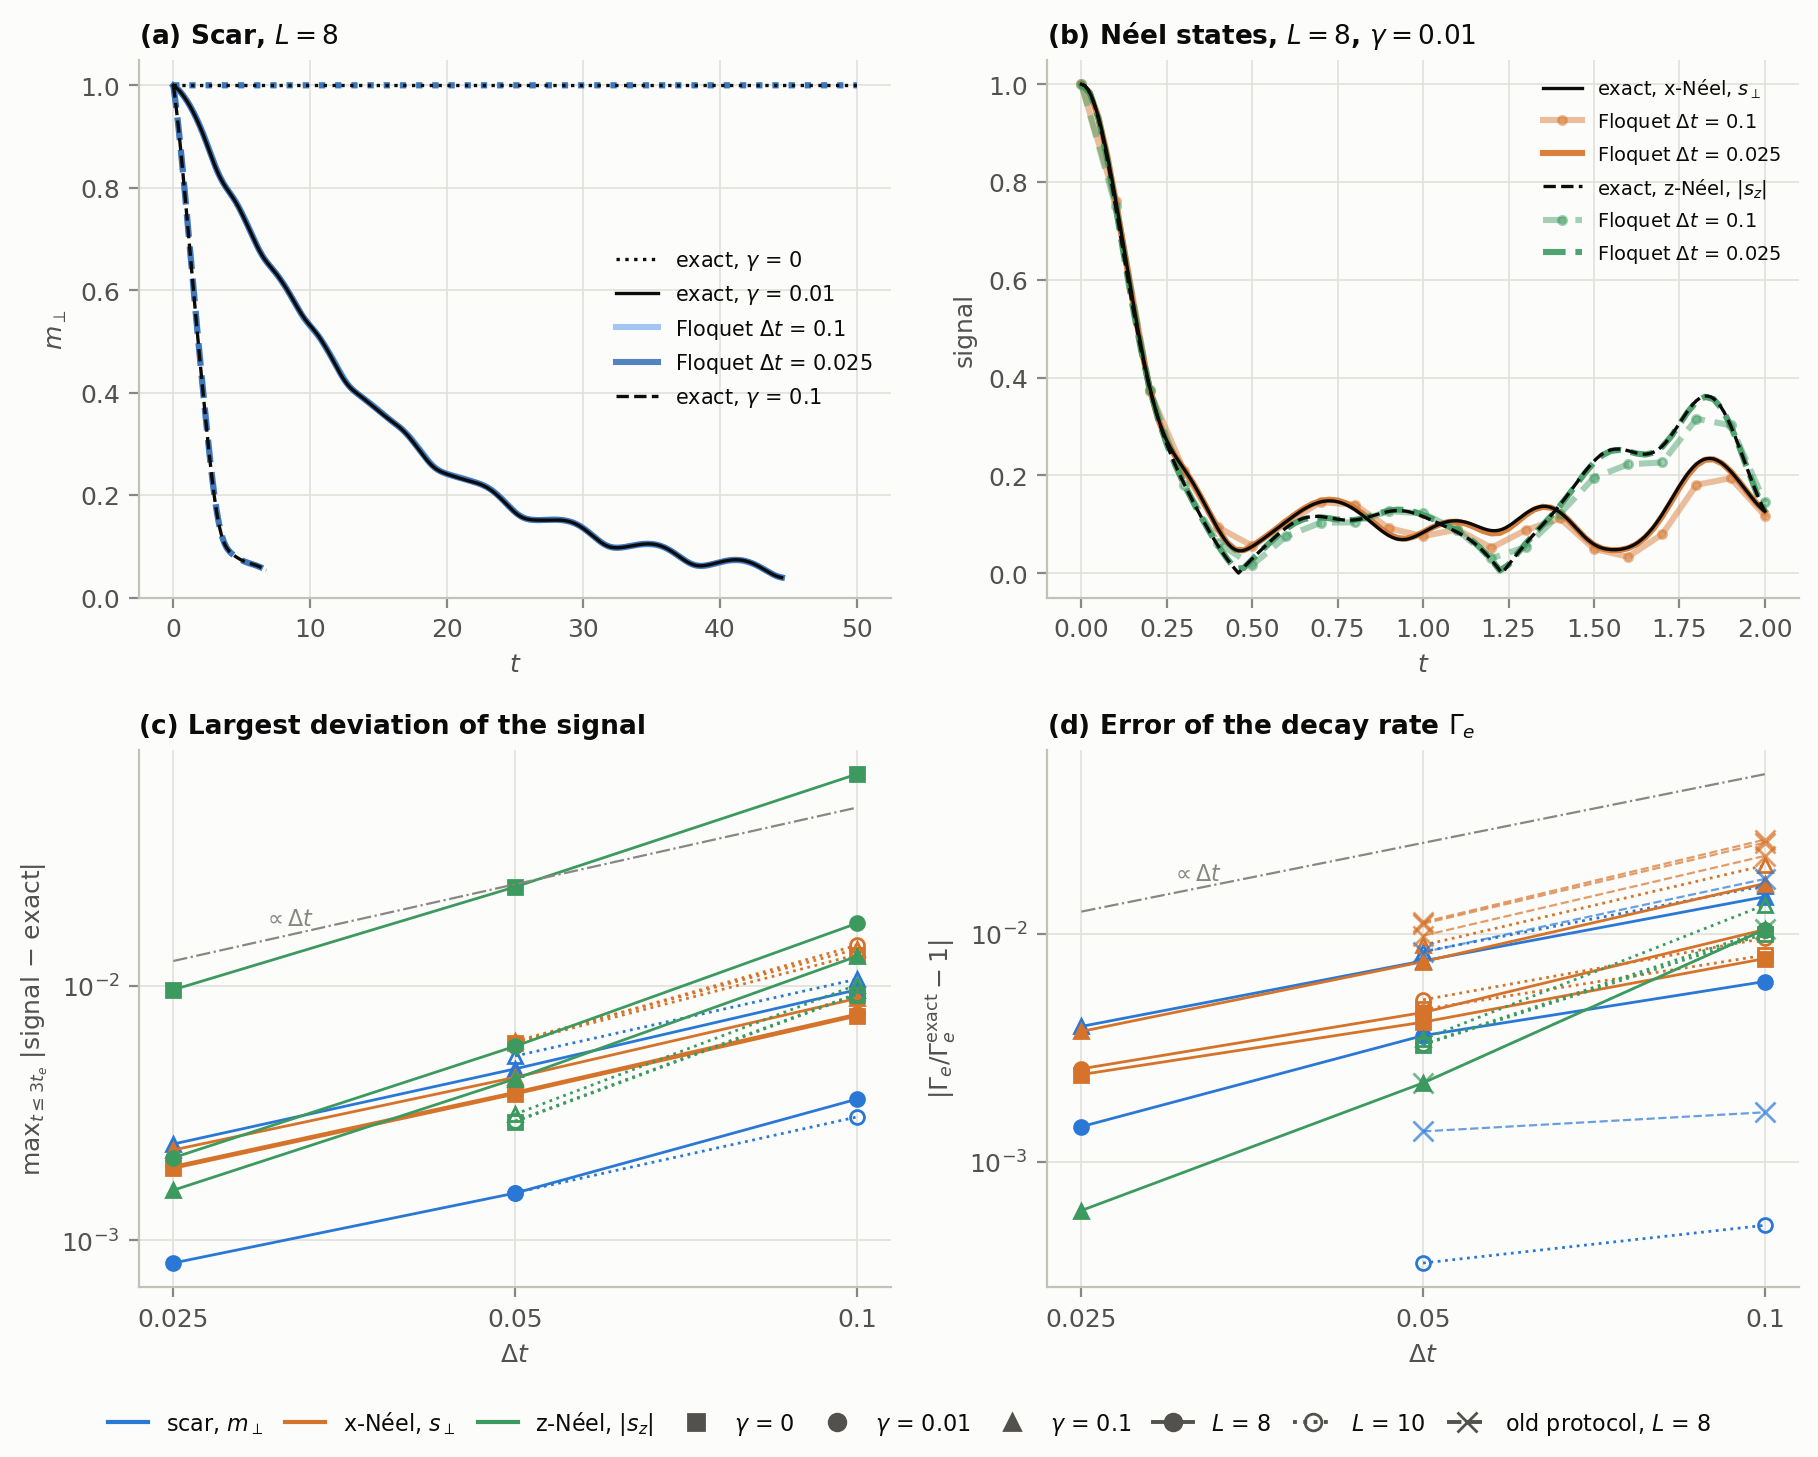
\includegraphics[width=\textwidth]{figures/floquet_checks.png}
\caption{Floquet circuit against the exact evolution ($\sigma^z$ noise). (a) Scar $m_\perp$ at $L = 8$: exact (black) and Floquet $\Delta t = 0.1$, $0.025$ (blue) at $\gamma = 0$ (dotted, $t \le 50$), $0.01$ (solid) and $0.1$ (dashed), each to $3t_e$. (b) x-Néel $s_\perp$ and z-Néel $|s_z|$ at $L = 8$, $\gamma = 0.01$, $t \le 2$; Floquet $\Delta t = 0.1$ with points at its output times. (c) Largest deviation of the signal over $t \le 3t_e$ (z-Néel at $L = 8$, $\gamma = 0$: the whole exact run, $t \le 5$) against $\Delta t$; filled $L = 8$, open $L = 10$; the $\gamma = 0$ scar ($\le 6\times10^{-13}$) is not shown. (d) Relative error of $\Gamma_e$, with the old protocol (crosses, $L = 8$); without the z-Néel state at $L = 8$, $\gamma \le 0.01$ (revival at the threshold, see text). Dash-dotted: $\propto\Delta t$. \texttt{plot\_scripts/floquet\_checks.py}, runs in \texttt{data/floquet/}.}
\label{fig:floquet-checks}
\end{figure}

\subsection{Depolarizing noise: thermodynamic decay rates}
\label{sec:floquet-dep}

With the circuit, the depolarizing panel of Fig.~\ref{fig:chinf} is recomputed with sizes up to $L = 24$ (20 there). The circuit approximates the Lindblad evolution
\begin{equation}
\dot\rho = \Lv(\rho) = -i[H,\rho] + \gamma\sum_{j=1}^{L}\sum_{\alpha = x,y,z}\big(\sigma^\alpha_j\,\rho\,\sigma^\alpha_j - \rho\big)
 = -i[H,\rho] + 4\gamma\sum_{j=1}^{L}\Big(\frac{\mathds 1_j}{2}\otimes\Tr_j\rho - \rho\Big),
\label{eq:floquet-dep}
\end{equation}
\begin{equation}
H = \sum_{j=1}^{L}\Big[\sum_{\alpha}\big(R_{j,j+1}\,\sigma^\alpha_{j+2} + \sigma^\alpha_{j-1}\,R_{j,j+1}\big) + \sum_{\alpha} c^{(j)}_{\alpha}\,\sigma^\alpha_{j-1}\,R_{j,j+1}\,\sigma^\alpha_{j+2}\Big] + \frac h2\sum_{j=1}^{L}\sigma^z_j ,
\label{eq:floquet-dep-H}
\end{equation}
i.e.\ the Hamiltonian of Sec.~\ref{sec:model} with its coefficients ($a = b = (1, 1, 1)$, $c_{\alpha\beta} = c^{(j)}_\alpha\,\delta_{\alpha\beta}$ with $c^{(j)}_\alpha$ uniform in $[0.5, 1.5]$, the realization of seed 1, $h = 1$, periodic ring) and the jump operators $\sqrt\gamma\,\sigma^\alpha_j$, $\alpha = x, y, z$, on every site. $\Tr_j$ is the partial trace over site $j$, so the last form replaces site $j$ by $\mathds 1_j/2$ at rate $4\gamma$: every Pauli factor of $\rho$ decays at $4\gamma$, and a free spin ($H_I = 0$) has $m_\perp = e^{-4\gamma t}$. This is the convention of Sec.~\ref{sec:kjma}, Eq.~\eqref{eq:kjma-dep}. Table~\ref{tab:channels} and Fig.~\ref{fig:chinf} use $\gamma_{\mathrm{dep}} = 2\gamma$ (jumps $\sqrt{\gamma_{\mathrm{dep}}/2}\,\sigma^\alpha_j$, channel \texttt{dep} in the code, Pauli factors at $2\gamma_{\mathrm{dep}}$). The runs below use \texttt{--channel dep} at $\gamma_{\mathrm{dep}} = 0.01, 0.02, 0.05, 0.1, 0.2, 0.5, 1, 2, 5, 10, 20$ and are quoted at $\gamma = \gamma_{\mathrm{dep}}/2 = 0.005, \dots, 10$; the rates $\Gamma$ do not depend on the convention.

\paragraph{Circuit and runs.} One step is Eq.~\eqref{eq:floquet-step} with $d = 4$ (every size used is divisible by 4, so the circuit is the same at every $L$). The noise layer multiplies the $\sigma^x_j$, $\sigma^y_j$ and $\sigma^z_j$ components of $\rho$ by $e^{-4\gamma\Delta t}$, i.e.\ on each site $\rho \to (1-q)\rho + (q/3)\sum_\alpha\sigma^\alpha_j\rho\,\sigma^\alpha_j$ with $q$ of Eq.~\eqref{eq:kjma-q}. $\Delta t = 0.1$ for the scar and $0.02$ for the Néel states; Trotter step $\Delta t\cdot\min(1, 0.25/\gamma)$ (the $\min(1, 0.5/\gamma_{\mathrm{dep}})$ of Sec.~\ref{sec:floquet-step}). States and signals as in Sec.~\ref{sec:states}: scar $m_\perp$, z-Néel $|s_z|$, x-Néel $s_\perp$, random $c$ of seed 1 (the realizations of the exact runs). \texttt{floquet} ($\rho$): $L = 8, 12$ at every $\gamma$ and $L = 16$ at $\gamma \le 1$, each also at $\Delta t/2$. \texttt{floquet\_traj}: $L = 16, 20, 24$, 224 trajectories, $\gamma \le 0.05$; at $L = 16$ only as a check, since $\rho$ is used where it exists. The runs stop at $2t_1$, $t_1$ the start of the latest stretch below $1/e$ (Néel $\rho$ at $L \le 12$, $\gamma \le 0.1$: to $t = 2.5$). Leonardo, 2026-11-26 (\texttt{data/bashes/floquet/make\_floquet\_dep\_jobs.sh}), data in \texttt{data/floquet\_dep/}.

\paragraph{Rates.} $\Gamma_e$ as in App.~\ref{sec:rates}, on each run's own output grid (trajectories with their statistical error). $\Ginf$ is $A$ of $\Gamma_e = A + B/L$ (unweighted) on $L = 8, 12, 16, 20, 24$ at $\gamma \le 0.05$ and on $L = 8, 12, 16$ at $0.1 \le \gamma \le 1$, the z-Néel state without $L = 8$ at $\gamma \le 0.01$ (finite-size revivals, as in Sec.~\ref{sec:channels-res}). Its error is the larger of the fit error and the change of $A$ when the smallest size is dropped. At $\gamma \ge 2.5$ there are only $L = 8, 12$, whose $\Gamma_e$ agree to $0.15\,\%$: $\Ginf = \Gamma_e(L = 12)$, with error $|\Gamma_e(12) - \Gamma_e(8)|$. The exact values are those of Fig.~\ref{fig:chinf} (exact $\rho$ at $L = 8, 10, 12$, diffusive trajectories at $L = 16, 20$ for $\gamma \le 1$).

\paragraph{Result.} Figure~\ref{fig:floquet-dep}. The scar rate grows from $\Ginf = 0.130 \pm 0.005$ at $\gamma = 0.005$ to the free-spin rate $4\gamma$ ($40.02$ at $\gamma = 10$). The Néel states stay at their closed-system thermalization rate up to $\gamma \approx 0.25$ (x-Néel $4.63$--$4.75$, z-Néel $4.97$--$5.19$) and join $4\gamma$ above $\gamma \approx 1$ ($40.36$ and $40.33$ at $\gamma = 10$). Floquet and exact $\Ginf$ agree within $1.2$ combined errors at every $\gamma$ for all three states. The one exception is the scar at $\gamma = 0.25$: $1.219 \pm 0.013$ against $1.251 \pm 0.007$ ($-2.6\,\%$, $2.2\sigma$). Relative differences at $\gamma \le 1$: scar $-4.7$ to $+3.2\,\%$, x-Néel $-2.9$ to $+1.8\,\%$, z-Néel $-1.9$ to $-6.7\,\%$. At $\gamma \ge 2.5$ they are below $0.6\,\%$ for all three states.

\paragraph{Where the differences come from.} Per size the circuit is close to exact. For this comparison the Floquet signal is sampled at the output times of the exact run of the same $(L, \gamma)$: the exact runs have output step 0.1 up to $\gamma \approx 0.25$, coarse against the Néel $t_e \approx 0.2$, and that biases the interpolated $1/e$ crossing. At $L = 8, 12$ (exact $\rho$ on both sides) the $\Gamma_e$ then differ by $0$ to $-2.0\,\%$ (scar), $0$ to $+0.6\,\%$ (x-Néel) and $0$ to $+0.3\,\%$ (z-Néel). The z-Néel offset of $\Ginf$ is therefore not the circuit but the set of sizes. The random-$c$ realization puts $L = 20$ about $4\,\%$ above $L = 12, 16$ ($\Gamma_e = 5.18$ against $4.98$ at $\gamma = 0.005$; the same realization effect as in Sec.~\ref{sec:channels-res}) and $L = 24$ about $3\,\%$ below ($4.84$), and the exact fit has $L = 20$ but no $L = 24$. Fitted on the common sizes ($L = 8, 12, 16, 20$; $12, 16, 20$ at $\gamma \le 0.01$), with the Floquet signal on the exact grid, the two z-Néel $\Ginf$ agree to $-0.9$ to $+1.0\,\%$ ($5.432$ against $5.431$ at $\gamma = 0.005$). For the scar the per-size difference is the Trotter error (next paragraph), and the $\gamma = 0.25$ outlier is that error ($-1.9\,\%$ per size) carried into $A$.

\paragraph{Trotter error.} The $\Delta t/2$ runs ($\rho$, $L = 8, 12, 16$) give $\Gamma_e(\Delta t)/\Gamma_e(\Delta t/2) - 1$, nearly the same at the three sizes. Scar: $-0.1$ to $-0.4\,\%$ at $\gamma \le 0.01$, then $-0.6$, $-0.8$, $-1.0$, $-0.9$, $-0.35$, $-0.15\,\%$ at $\gamma = 0.025$, $0.05$, $0.1$, $0.25$, $0.5$, $1$, and at most $0.04\,\%$ at $\gamma \ge 2.5$. Néel states: $+0.002$ to $+0.29\,\%$, largest at $\gamma = 0.25$. The step is first order, so $\Gamma_e(\Delta t) - \Gamma_e(0) \approx 2[\Gamma_e(\Delta t) - \Gamma_e(\Delta t/2)]$. That is about $-1.5$ to $-2\,\%$ for the scar at $\gamma = 0.05$--$0.25$ ($\Delta t = 0.1$; the Trotterized scar decays slightly slower, as under $\sigma^z$ noise in Sec.~\ref{sec:floquet-checks}) and at most $+0.6\,\%$ for the Néel states ($\Delta t = 0.02$). It matches the per-size difference from exact above (scar $-1.6$ to $-2.0\,\%$ at the same $\gamma$). At large $\gamma$ the step shrinks as $\Delta t/(4\gamma)$ and the decay is set by the noise layer, which is exact, so the error vanishes.

So with $\Delta t = 0.1$ (scar) and $0.02$ (Néel states) the circuit gives the depolarizing $\Ginf$ of Fig.~\ref{fig:chinf} within its errors, up to $L = 24$. Its own error is the first-order Trotter error: at most $2\,\%$ for the scar and $0.6\,\%$ for the Néel states.

\begin{figure}[H]
\centering
\includegraphics[width=0.75\textwidth]{floquet_dep_thermodynamic_rate.png}
\caption{Depolarizing noise, Eq.~\eqref{eq:floquet-dep}: $\Ginf$ against $\gamma$ (jumps $\sqrt\gamma\,\sigma^\alpha_j$) for the scar ($m_\perp$), the z-Néel ($|s_z|$) and the x-Néel state ($s_\perp$). Filled: Floquet circuit ($\Delta t = 0.1$ scar, $0.02$ Néel; $A + B/L$ on $L = 8$--$24$ at $\gamma \le 0.05$ and $8$--$16$ at $0.1$--$1$, $\Gamma_e(L = 12)$ at $\gamma \ge 2.5$). Open: exact Lindblad evolution, the depolarizing panel of Fig.~\ref{fig:chinf} with $\gamma = \gamma_{\mathrm{dep}}/2$. Dotted: free spin, $4\gamma$ (\texttt{plot\_scripts/floquet\_dep\_rates.py}, runs in \texttt{data/floquet\_dep/}).}
\label{fig:floquet-dep}
\end{figure}
